%! program = pdflatex

%
%  Master Thesis von Dirk Breuer
%
%  Created by Dirk Breuer on 2008-06-02.
%  Copyright (c) 2008 Dirk Breuer. All rights reserved.
%
% only4mac: makeindex Master\ Thesis.nlo -s nomencl.ist -o Master\ Thesis.nls

% header inkludieren. Beinhaltet Pakete und Layoutanweisungen
%!TEX root = /Users/dbreuer/Documents/Work/_FH/_Master/master_thesis/Main/Master Thesis.tex

%%% PREAMBLE

\documentclass[12pt,
               headsepline,
               DIV14, % Seitenränder festlegen
               BCOR5mm, % Bindekorrektur
               a4paper,
               oneside,
               cleardoublestandard,
               openany,
               bibtotoc,
               liststotoc,
               halfparskip,
               pointlessnumbers,
               final
               ]{scrbook}

% Paket für Zeilenabstände
\usepackage{setspace}
\raggedbottom

\usepackage{scrpage2}
\pagestyle{scrheadings}
\clearscrheadfoot
\cfoot{\pagemark}
% \ihead{\headmark}
\ohead{\headmark}
% \automark{section}

% include XMP-Metadata
\usepackage{xmpincl} 
\includexmp{std/metadata}

% Wie viele Ebenen im Inhaltsverzeichnis?
\setcounter{tocdepth}{3}

% Bis zu welcher Ebene sollen die Abschnitt nummeriert werden
\setcounter{secnumdepth}{3}

% Grafiken und Farbe
\usepackage[pdftex]{graphicx} % for graphic handling
\usepackage[usenames,dvipsnames,pdftex]{color} % for color handling
% Einige Farben
\definecolor{lightgray}{gray}{0.9}
\definecolor{cmd_line}{rgb}{0.4,.8,1}
\definecolor{comment}{rgb}{0.2,0.7,0.5}

% Paket für Rotation
\usepackage{rotating}

% Paket für Listings
\usepackage{listings}
\usepackage{dvsm} % Use DejaVu Sans Mono as Monospace Font
% get closed frames on each page for listings
\usepackage{framed}
\newenvironment{kasten}{%
  \def\FrameCommand{\fboxsep=\FrameSep \colorbox{lightgray}}%
  \MakeFramed {\hsize=0.9\textwidth \FrameRestore}}%
 {\endMakeFramed}

\lstloadlanguages{Java,XML,Ruby,HTML}
\newcommand{\listingname}{Listing}
\lstset{
  numbers=left, 
	numberstyle=\ttfamily\tiny, 
	stepnumber=1,
	lineskip=2pt,
	numbersep=5pt,
	language=Java,
	breaklines=true,
	breakautoindent=true,
	postbreak=\space,
	tabsize=2,
	frame=single,
  keywordstyle=\bfseries\color{blue},
  stringstyle=\color{ForestGreen},
	numberfirstline=false,
  commentstyle=\slshape\scriptsize\color{Gray},
  basicstyle=\ttfamily\scriptsize,
  % morekeywords={while,condition,invoke,receive,assign,pipe},
  keywordstyle=[2]\ttfamily\redhighlight,
  keywordstyle=[3]\ttfamily\yellowhighlight,
  keywordstyle=[4]\ttfamily\slshape
}

% bg colored text for highlighting

\newcommand{\redhighlight}[1]{\colorbox{red}{\textcolor{white}{#1}}}
\newcommand{\yellowhighlight}[1]{\colorbox{yellow}{\textcolor{black}{#1}}}

% Listings can be included as following:
% 
% include a file (from line n to m): \lstinputlisting[firstline=n,lastline=m]
% 
% standard listing: \begin{lstlisting} ... \end{lstlisting}
% 
% Inline: \lstinline+code here+

\lstdefinelanguage{YAML}{
  morekeywords = {uri, successors, type, output, namespace, description, predecessors, input},
  % moredelim=[is][\color{green}]{"},
  emph={[2]null},
  emphstyle=[2]\bfseries\color{red},
  moredelim=[l][\color{OliveGreen}]{"},
  morecomment=[l][commentstyle]{\#},
}
% 
% \lstdefinelanguage{Turtle}{
%     morekeywords = {@prefix},
%   emphstyle=\itshape %\underbar
%   % emph={[2]mit,sonst},
%   % emphstyle=[2]\color{red},
%   % moredelim=[is][\color{green}]{/*}{*/}
% }

% Use utf-8 encoding for foreign characters
\usepackage[utf8]{inputenc}

% Paket das die Ausgabefonts definiert
% \usepackage[T1]{fontenc}

% Paket um jede Schriftgröße zuzulassen
% \usepackage{type1cm}

% This is now the recommended way for checking for PDFLaTeX:
\usepackage{ifpdf}

% change enumeration package
\usepackage{enumerate}

% Package for verbatim text
% \usepackage{verbatim}
% Notwendiges Paket, um Verbatim in Fußzeilen zu setzen
% \usepackage{fancyvrb}
% \VerbatimFootnotes

% schoenere Kennzeichnung im Literaturverzeichnis
\usepackage[square,sort]{natbib}
% Festlegung Art der Zitierung - Havardmethode: Abkuerzung Autor + Jahr %
% BibTeX Style nach Norm DIN 1505 %
\bibliographystyle{natdin}

% Schriftstile umsetzen
% \setkomafont{sectioning}{\normalfont\normalcolor\bfseries}
\setkomafont{descriptionlabel}{\normalfont\normalcolor\bfseries}
\setkomafont{captionlabel}{\usekomafont{descriptionlabel}}
\setkomafont{dictumtext}{\normalfont\normalcolor\itshape}
\setkomafont{dictumauthor}{\scshape}

% Hurenkinder und Schusterjungen verhindern
\clubpenalty = 10000
\widowpenalty = 10000
\displaywidowpenalty = 10000

% Paket für die Verwendung von URLs durch den Befehl \url{}
\usepackage{url}

%\usepackage{array}
\usepackage{colortbl}

% Babelpaket für deutsche Bezeichner
\usepackage[ngerman]{babel}

% For syntax Checking
\usepackage{syntonly}
% \syntaxonly % Comment out for Output

\usepackage{makeidx}
% \makeindex

% Mathepakete
\usepackage{amssymb} %maths
\usepackage{amsmath} %maths
\usepackage{amsthm}

% Mathematische Definition
\newtheorem{definition}{Definition}
% \usepackage{mathabx}

% Springt im PDFViewer an die Stelle an der gerade editiert wurde
\usepackage{pdfsync}

% Paket und Einstellungen für das Abkürzungsverzeichnis
\usepackage[norefpage,noprefix,german,intoc]{nomencl}
% Befehl umbenennen in abk
\let\abk\nomenclature
% Deutsche Überschrift
\renewcommand{\nomname}{Abkürzungsverzeichnis}
% Punkte zw. Abkürzung und Erklärung
\renewcommand{\nomlabel}[1]{#1 \dotfill}
% Zeilenabstände verkleinern
\setlength{\nomitemsep}{-\parsep}
% Definiert die Aufteilung im Glossar zwischen Begriffen und Erläuterung
\setlength{\nomlabelwidth}{.25\hsize}
%\makeglossary
\makenomenclature

%Paket für ein deutsches Literaturverzeichnis
\usepackage{bibgerm}

% other commands
\newcommand{\note}[1]{\textbf{#1}}

\pdfpagewidth=\paperwidth \pdfpageheight=\paperheight
\usepackage[pdftex,plainpages=false,pdfpagelabels,
            pdftitle={Konzeption, prototypische Realisierung und szenariobasierte Validierung einer dienstorientierten Multimediaarchitektur},
            pdfauthor={Dirk Breuer - University of Applied Science, Cologne},
            pdfkeywords={Architektur,SOA,Prototyping,COSIMA,Validierung}]{hyperref} % Has to stand at the end of the preamble

%%% END PREAMBLE


%%% BEGIN DOCUMENT
\begin{document}

% Vermeidung von "duplicate page" Fehlern
% siehe: http://theoval.sys.uea.ac.uk/~nlct/latex/pdfdoc/pdfdoc/pdfdoc.html
\pagenumbering{alph}

% Unbeschriftetes Vorblatt
\include{std/empty}

 % Titelseite einbinden
%!TEX root = /Users/dbreuer/Documents/Work/_FH/_Master/master_thesis/Main/Master Thesis.tex

\begin{titlepage}

\begin{center}

%Logo der Fachhochschule Köln
\begin{figure}[!ht]
	\flushleft
		\includegraphics[natwidth=920pt, natheight=95pt, width=.5\textwidth]{images/fh_logo.pdf}
\end{figure}

\vspace{0.5cm}

% Master Thesis 
\begin{Large}
  \textsc{Master Thesis}\\[0.7em]
\end{Large}

%Deutscher Titel
\begin{rmfamily}
  \LARGE
  \textbf{
  Konzeption, prototypische Realisierung und szenariobasierte Validierung einer dienstorientierten Multimediaarchitektur
  }\\
\normalsize
\end{rmfamily}

\vspace{0.5cm}

%Englischer Titel
% \begin{rmfamily}
% \textbf{\LARGE Title in English}\\
% \large with a very\\long subtitle\\
% \normalsize
% \end{rmfamily}
% 
% \vspace{1.2cm}

%ausgearbeitet von...
% \begin{large}
ausgearbeitet von\\ 
% \vspace{0.2cm}
\begin{Large}
Dirk Breuer, 11038920\\Medieninformatik Master\\
\end{Large}
% \end{large}

\vspace{0.6cm}

%zur Erlangung des akademischen Grades...
zur Erlangung des akademischen Grades\\
% \vspace{0.2cm}
\begin{large}
\textsc{Master of Science}\\ 
\end{large}

\vspace{0.4cm}

%vorgelegt an der...
vorgelegt an der\\ 
% \vspace{0.2cm}
\begin{large}
\begin{scshape}
Fachhochschule Köln\\
University of Applied Sciences Cologne\\
Fakultät für Informatik und\\
Ingenieurwissenschaften\\
\end{scshape}
\end{large}

\vspace{0.4cm}

%im Studiengang...
\vspace{0.2cm}
im Studiengang\\ 
\begin{large}
\textsc{Medieninformatik (Master)}
\end{large}

\vspace{0.7cm}

%Autor der Bachelorarbeit und die Prüfer
\begin{tabular}{rl}
         Erster Prüfer: &  Prof. Dr. Mario Winter\\
       							    &  \small Fachhochschule Köln \\[1.0em]
        Zweiter Prüfer: &  Prof. Dr. Kristian Fischer\\
       							    &  \small Fachhochschule Köln \\
\end{tabular}

\vspace{0.5cm}

%Ort, Monat der Abgabe
% \begin{large}
\textsc{Gummersbach, im Dezember 2008}
% \end{large}

\end{center}

\newpage
\thispagestyle{empty}

%Kontaktmöglichkeiten des Autors und der Prüfer
\begin{center}
\begin{tabular}{rl}
							&  \\[34.0em]
							
\large \textbf{Adressen:}	&  \quad Dirk Breuer\\
							&  \quad Redwitzstr. 6\\
							&	 \quad 50937 Köln\\
							&  \quad dirk.breuer@gmail.com\\[2.0em]
							
							&  \quad Prof. Dr. Mario Winter\\
							&  \quad Fachhochschule Köln\\
							&  \quad Institut für Informatik\\
							&	 \quad Steinmüllerallee 1\\
							&  \quad 51643 Gummersbach\\
							&  \quad mario.winter@fh-koeln.de\\[2.0em]
							
							&  \quad Prof. Dr. Kristian Fischer\\
							&  \quad Fachhochschule Köln\\
							&  \quad Institut für Informatik\\
							&	 \quad Steinmüllerallee 1\\
							&	 \quad 51643 Gummersbach\\
							&  \quad kristian.fischer@fh-koeln.de\\
\end{tabular}
\end{center}

\end{titlepage}


\frontmatter

% Einbinden des Inhaltsverzeichnis
\tableofcontents

% Einbinden des Abstracts bzw. der Kurzfassung
%!TEX root = /Users/dbreuer/Documents/Work/_FH/_Master/master_thesis/Main/Master Thesis.tex

\chapter*{} % (fold)

\begin{center}
\huge \textbf{Abstract}\\
\end{center}
\vspace{1cm}
\normalsize

Lorem ipsum dolor sit amet, consectetur adipisicing elit, sed do eiusmod tempor incididunt ut labore et dolore magna aliqua. Ut enim ad minim veniam, quis nostrud exercitation ullamco laboris nisi ut aliquip ex ea commodo consequat. Duis aute irure dolor in reprehenderit in voluptate velit esse cillum dolore eu fugiat nulla pariatur. Excepteur sint occaecat cupidatat non proident, sunt in culpa qui officia deserunt mollit anim id est laborum.

\vspace{2cm}
\begin{center}
\huge \textbf{Zusammenfassung}\\
\end{center}
\vspace{1cm}
\normalsize

Lorem ipsum dolor sit amet, consectetur adipisicing elit, sed do eiusmod tempor incididunt ut labore et dolore magna aliqua. Ut enim ad minim veniam, quis nostrud exercitation ullamco laboris nisi ut aliquip ex ea commodo consequat. Duis aute irure dolor in reprehenderit in voluptate velit esse cillum dolore eu fugiat nulla pariatur. Excepteur sint occaecat cupidatat non proident, sunt in culpa qui officia deserunt mollit anim id est laborum.

% Einbinden des Abbildungsverzeichnis %
\listoffigures

% Einbinden des Tabellenverzeichnis %
\listoftables

% Einbinden des Listingverzeichnis %
\lstlistoflistings

% Einbinden des Abkürzungsverzeichnis %
\printnomenclature

% Einbinden des Stichwortverzeichnis %
%\renewcommand{\indexname}{Stichwortverzeichnis}
%\printindex

\mainmatter

% 1 1/2-facher Zeilenabstand im Hauptteil
\onehalfspacing

%!TEX root = /Users/dbreuer/Documents/Work/_FH/_Master/master_thesis/Main/Master Thesis.tex

\chapter{Einleitung} % (fold)
\label{cha:einleitung}

  Im Titel der vorliegenden Arbeit wird bereits herausgestellt, dass eine Architektur von der Konzeption über die prototypische Implementierung bis hin zu einer ersten Validierung betrachtet wird. Dabei soll die Architektur dienstorientiert aufgebaut sein und sich für die Realisierung von Multimediaanwendungen eignen.
  
  In dieser Arbeit wird dazu zunächst allgemein in die Thematik der Dienstorientierung eingeführt und die jeweiligen Besonderheiten im Zusammenhang mit Multimediaanwendungen dargelegt. Im weiteren Verlauf wird die Architektur prototypisch umgesetzt und auf Grund der Implementierung eines Anwendungsszenarios validiert.

\section{Motivation} % (fold)
\label{sec:motivation}

  Die Motivation zu dieser Arbeit ist durch das COSIMA\abk{COSIMA}{Cologne Service-Oriented Integrated Multimedia Architecture}-Projekt begründet, welches im Rahmen des Wahlpflichtfaches \emph{Modellierung in audio-visuellen Medien} an der Fachhochschule Köln entstanden ist. Das COSIMA-Projekt soll eine verteilte, dienstorientierte Architektur zur Realisierung von Multimediaanwendungen zum Ergebnis haben.
  
  Da bis zu diesem Zeitpunkt ausschließlich konzeptionell an diesem Projekt gearbeitet wurde, bestand der dringende Bedarf einer ersten prototypischen Implementierung und eine anschließende Validierung des bis dato Konzipierten durchzuführen. Da COSIMA als langfristiges Projekt ausgelegt ist, ist es zu diesem Zeitpunkt notwendig, eine erste Überprüfung durchzuführen, bevor weitere konzeptionelle Arbeiten vorgenommen werden.
  
  Das szenariobasierte Vorgehen, dass der Validierung zu Grunde liegt, wurde motiviert durch die Neuartigkeit des Projekts und der damit verbundenen Unerfahrenheit bei der Konstruktion entsprechender Anwendungen. Der Einsatz von Szenarien soll helfen, diese Unerfahrenheit zu einem gewissen Grad zu kompensieren.

% section motivation (end)

\section{Zielsetzung und Aufgabenstellung} % (fold)
\label{sec:zielsetzung_und_aufgabenstellung}

  Diese Arbeit verfolgt zwei wesentliche Ziele, von denen sich eines direkt aus dem Titel ableiten lässt, das andere ergibt sich aus dem COSIMA-Projekt selbst:

  \begin{enumerate}
    \item Es soll überprüft werden, inwiefern sich die bis zu diesem Zeitpunkt konzipierte Architektur von COSIMA für den Einsatz als dienstorientierte Architektur für Multimediaanwendungen eignet. 
    \item Das zweite Ziel ist, dass die Ergebnisse dieser Arbeit, vor allem die prototypische Implementierung, einen Rahmen für weitere Arbeiten geben sollen.
  \end{enumerate}
  
  Diese Ziele werden operationalisiert und ergeben damit konkrete Aufgaben, die es im Rahmen dieser Arbeit zu erfüllen gilt. Die Erledigung der einzelnen Aufgaben hat dementsprechend die Zielerreichung zur Folge. Am Ende dieser Arbeit kann jedoch keine binäre Aussage über die Vollständigkeit oder Korrektheit der durchgeführten Implementierung getroffen werden, denn auch Teilergebnisse müssen dabei berücksichtigt bleiben.
  
  Zunächst ist es notwendig die konzipierte Architektur und ihre wesentlichen Komponenten im Einzelnen vorzustellen und zu diskutieren. Daraus lassen sich die einzelnen Elemente ableiten, die später implementiert werden müssen.
  
  Um überhaupt eine Aussage über die Eignung der Architektur für die Umsetzung von Multimediaanwendungen treffen zu können, muss eine entsprechende Anwendung realisiert werden. Zu diesem Zwecke wird zunächst ein Szenario entwickelt, in dem diese Anwendung eingebettet wird. Zur Realisierung dieser Anwendung muss demzufolge zunächst die Architektur selbst implementiert werden.
  
  Am Ende wird somit ein Prototyp der Architektur entstanden und das Szenario entsprechend umgesetzt sein. An diesem Punkt lässt sich feststellen, ob sich die Architektur für den geplanten Einsatz eignet oder nicht.
  
  Für die Erreichung des zweiten Ziels ist vor allem notwendig, dass die Implementierung so ausgeführt und dokumentiert wird, dass nachfolgende Arbeiten nach kurzer Einarbeitungszeit darauf aufsetzen können. Das Szenario sollte so breit ausgelegt sein, dass es ebenfalls für weitere Arbeiten als Grundlage dienen kann.
  
% section zielsetzung_und_aufgabenstellung (end)

\section{Abgrenzung} % (fold)
\label{sec:abgrenzung}

  In der vorliegenden Arbeit soll das COSIMA-Projekt und dessen Architektur horizontal betrachtet und implementiert werden. Es fand keine detaillierte Einzelbetrachtung bestimmter Charakteristika, wie etwa \emph{Synchronisation} oder \emph{Streaming} statt. Aus diesem Grund ist das Ergebnis auch nicht eine vollständige Umsetzung der Gesamtarchitektur, wohl wurde aber eine solide Implementierung geschaffen, die es weiterführenden Projekten erlaubt, bestimmte Bereiche vertikal zu implementieren. Ebenso konnten nicht-funktionale Aspekte wie etwa \emph{Skalierbarkeit} oder \emph{Wartbarkeit} keine Berücksichtigung finden.

% section abgrenzung (end)

\section{Aufbau der Arbeit} % (fold)
\label{sec:aufbau_der_arbeit}

  Zunächst wird in das COSIMA-Projekt eingeführt und die Konzeption der zugrunde liegenden Architektur vorgestellt ($\to$ Kapitel \ref{cha:eine_dienstorientierten_multimediaarchitektur}). In diesem Zuge werden ebenfalls die zentralen Begriffe \emph{Architektur}, \emph{Dienstorientierung} und \emph{Multimedia} definiert.
  
  Im Anschluss daran wird eine Einführung in szenarienbasiertes Vorgehen im Allgemeinen gegeben und im Speziellen welche Methode in dieser Arbeit verwendet wurden. Des Weiteren wird das Szenario vorgestellt, gegen das die prototypische Realisierung validiert werden soll ($\to$ Kapitel \ref{cha:szenario}).
  
  Im nachfolgenden Kapitel werden sowohl die prototypische Implementierung der Architektur von COSIMA selbst, als auch die Umsetzung des zuvor beschriebenen Szenarios auf Basis dieser Architektur ($\to$ Kapitel \ref{cha:prototypische_realisierung}) diskutiert.
  
  Die Ergebnisse und Erkenntnisse, die sich aus der Validierung der beiden Implementierungen ergeben haben, finden sich in Kapitel \ref{cha:validierung_der_architektur}. Hier findet zudem eine Einordnung des Begriffs \emph{Validierung} statt.
  
  Die Arbeit schließt mit einer Zusammenfassung und kritischen Bewertung der wesentlichen Aspekte. Ebenso wird an dieser Stelle ein Ausblick gegeben, welche nächsten Schritte als sinnvoll zu erachten sind, um das COSIMA-Projekt voranzutreiben ($\to$ Kapitel \ref{cha:fazit}).
  
% section aufbau_der_arbeit (end)

% chapter einleitung (end)
%!TEX root = /Users/dbreuer/Documents/Work/_FH/_Master/master_thesis/Main/Master Thesis.tex

\chapter{COSIMA - Eine dienstorientierten Multimediaarchitektur} % (fold)
\label{cha:eine_dienstorientierten_multimediaarchitektur}

  Im Abschnitt~\ref{sec:motivation} wurde bereits kurz darauf eingegangen, dass die vorliegenden Arbeit vor dem Hintergrund des COSIMA-Projekts entstanden ist. In diesem Kapitel soll dieses Projekt so weit vorgestellt werden, dass für den weiteren Verlauf der Arbeit ein grundlegendes Verständnis über die Ziele, Alleinstellungsmerkmale und Herausforderungen existiert.
  
\section{Motivation und Ziele von COSIMA} % (fold)
\label{sec:motivation_und_ziele_von_cosima}

  Das COSIMA-Projekt ist aus dem Wahlpflichtfach Modellierung in audio-visuellen Medien (MIAV\abk{MIAV}{Modellierung in audio-visuellen Medien}) an der Fachhochschule Köln im Masterstudiengang der Medieninformatik hervorgegangen. Im Rahmen einer Projektarbeit wurde das die Projektidee weiter ausgearbeitet und konzeptioniert. Die Ergebnisse dieser Arbeit wurden als Institutsbericht an Fachhochschule Köln bereitsgestellt und sind dort im Detail einsehbar~\citep{bericht}.
  
  Das folgende Kapitel wird daher nur auf die wesentliche Punkte des COSIMA-Projekts eingehen und ihre Relevanz für diese Arbeit herausstellen. Die ursprüngliche Idee hinter COSIMA war es ein Framework zu entwickeln, dass die Entwicklung von Multimediaanwendungen vereinfacht. Im Gegensatz zu anderen Medienframeworks, wie etwa dem \emph{Java Media Framework} (JMF\abk{JMF}{Java Media Framework}), wurde bei dem COSIMA-Projekt ein ganzheitlicher Ansatz verfolgt.
  
  Im Institutsbericht wird darauf hingewiesen, "`dass die Entwicklung von Multimediaanwendungen derzeit verhältnismässig aufwendig ist"'~\citep[S. 2]{bericht}. Eine Ursache dieser Problematik, liegt nach Aussage der Autoren darin begründet, dass sich die zur Zeit verfügbaren Rahmenwerke im Bereich der Multimediaverarbeitung auf einen sehr engen Einsatzbereich beschränken. Neben JMF sind hier zusätzlich noch \emph{QuickTime}\footnote{\url{http://www.apple.com/quicktime/}} und \emph{ImageJ}\footnote{\url{http://rsbweb.nih.gov/ij/}} zu nennen. Andere Aspekte von Multimediaanwendungen, wie etwa die Integration von Metadaten, müssten von dem Anwendungsentwickler erst manuell mit diesen Rahmenwerken integriert werden. "`Ein Meta-Framework, welches die bestehenden Ansätze verbinden und integrieren könnte, würde die Wiederverwendbarkeit und generelle Entwicklungsarbeit positiv beeinflussen, beziehungsweise vereinfachen"'~\citep[S. 3]{bericht}, wird von den Autoren des Berichts daher als Bestreben hinter dem COSIMA-Projekt angeführt.
  
  Neben der Notwendigkeit ein \emph{Meta-Framework}\footnote{Das ursprüngliche Ziel war tatsächlich ein Framework zu schaffen. Erst während der Validierung im Rahmen dieser Arbeit ist zu Tage gekommen, dass es sich mehr um eine Architektur handelt und weniger um ein Framework. Im weiteren Verlauf wird darauf jedoch noch genauer eingegangen.} zu schaffen, führen die Autoren als weiteren Beweggrund das Fehlen einer Architektur für Multimediaanwendungen an. Innerhalb dieser Architektur könnten sich Anwendungsentwickler wesentlicher effektiver bewegen und müssten nicht erst eine eigene Architektur von Grund auf entwerfen.
  
  Da sich mit den meisten bestehenden Multimedia-Rahmenwerke keine verteilten Anwendungen realisieren lassen, lag auch dieser Aspekt von Beginn an im Fokus der Konzeptionierung. Als Grundlage eine geeignete Architektur zu konzeptionieren, die es ermöglicht, verteilte Anwendungen zu realisieren, diente das Konzept der \emph{Service-oriented Architecture} (SOA\abk{SOA}{Service-oriented Architecture}) oder \emph{Dienst-orientierten Architektur}.
  
  Die hier aufgeführten Punkte haben initial die Entwicklung eines Rahmenwerkes motiviert, dass später im COSIMA-Projekt aufgehen sollte. Die im Verlauf der Projektarbeit entwickelten Ziele von COSIMA sind im nächsten Abschnitt zusammen gefasst.
  
\subsection{Ziele} % (fold)
\label{sub:ziele}

  Das \emph{Mission Statement} des COSIMA-Projekts fasst alle Ziele des Projekts in einer Kernaussage zusammen:

  \begin{quote}
    \emph{``MIAV ist ein integratives, komponentenbasiertes Meta-Framework mit gezielter Ausrichtung auf Multimediaverarbeitung. Es vereinfacht die Entwicklung von verteilten Multimedia-Applikationen durch eine flexible, dienst-orientierte Architektur. Die Wiederverwendbarkeit von Komponenten und bestehenden Frameworks wird dadurch begünstigt.''} (aus~\citep[S. 2]{bericht})\footnote{Die Bezeichnung "`COSIMA"' hat das Projekt erst nach Fertigstellung des Berichts erhalten, daher findest sich hier noch die zuvor verwandte provisorische Bezeichnung \emph{MIAV-Framework}.}
  \end{quote}

  Neben den zentralen Aspekten \emph{dienst-orientierte Architektur}, \emph{Integration} und \emph{Meta-Framework}, die im Abschnitt zuvor bereits dargestellt wurden, nennen die Autoren hier zusätzlich noch die Aspekte der \emph{komponentenbasierten Architektur}, \emph{Wiederverwendbarkeit} und natürlich der \emph{Medienverarbeitung}.
  
  Neben den hier genannten Zielen, die das COSIMA-Projekt zu erreichen versucht, zeichnet sich das Projekt durch seine spezifischen Charakteristika in Bezug auf andere Multimedia-Rahmenwerke aus. Diese Alleinstellungsmerkmale werden im nächsten Abschnitt genauer betrachtet.

  % - Welche Ziele verfolgt das COSIMA-Projekt?
  % - Warum handelt es sich um eine Architektur und nicht um ein Framework!!!! (Im Bericht noch anders, irgendwie muss das hier verwurstet werden!)
  % - Weiterentwicklung der Definition seit dem Bericht

% subsection ziele (end)
  
% section motivation_und_ziele_von_cosima (end)

\section{Alleinstellungsmerkmale} % (fold)
\label{sec:alleinstellungsmerkmale}

  Aus den in Abschnitt~\ref{sub:ziele} dargestellten Zielen des COSIMA-Projekts lassen sich die folgenden Merkmale extrahieren, die COSIMA im Bereich der Multimedia-Rahmenwerke und -Anwendungen einmalig machen~\citep[S. 3f]{bericht}:
  
  \begin{description}
    \item[Verteiltheit] COSIMA ist konzeptioniert als ein verteiltes System.
    \item[Dienstorientierung] Angelehnt an die \emph{Service-Oriented Architecture} (SOA), sind die Bausteine in COSIMA als Dienste modelliert.
    \item[Integration] Bestehende Frameworks können in Form von Diensten angeboten und so ihre Funktionalität eingebunden werden.
    \item[Erweiterbarkeit] Die Dienstorientierung erlaubt die Einbindung eigener Komponenten.
    % TODO - Die Skalierbarkeit muss hier noch weiter beschrieben werden. Eine reine Verteilung führt noch zu keiner gute Skalierbarkeit eines Systems.
    \item[Skalierbarkeit] Als verteiltes System können Dienste auf verschiedene Systeme ausgelagert werden, es gibt kein monolithisches System\footnote{die Verschiebung des Flaschenhalses von einem System hat zur Folge, dass die Verbindung zwischen den Diensten entsprechend angelegt sein muss. [\textbf{QUELLE}]}.
    \item[Medienobjekt-Modellierung] Modellierung von Medien in ganzheitlicher Betrachtungsweise von Rohdaten und Metadaten in einem Objekt.
    \item[Meta-Ebene] COSIMA fokussiert nicht auf Datensicht oder Metadatensicht sondern abstrahiert auf höhere Ebene.
    \item[Medienverarbeitung] Ganzheitliche Sicht auf Medienverarbeitung: Produktion, Verarbeitung, Transformation, Anreicherung, Wiedergabe, Ausgabe von Daten und Metadaten
    \item[Architektur] COSIMA stellt eine Architektur für Multimediaanwendungen
  \end{description}

% section alleinstellungsmerkmale (end)

\section{Architektur} % (fold)
\label{sec:architektur}

  - Vorstellen der Architektur
  - Kurze Historie der Architektur und Entwicklung bis jetzt!
  - Konzept darstellen (kurz), dabei verweisen auf den Bericht
  
\subsection{zentrale Komponenten} % (fold)
\label{sub:zentrale_komponenten}

  - Kernpunkte der Architektur herausarbeiten
  - Diese Kernpunkte müssen in der Realisierung/Validierung entsprechend besondere Berücksichtigung finden
  
\subsubsection{Kernkomponenten} % (fold)
\label{ssub:kernkomponenten}

   - Zentrale Komponente der Architektur erläutern
   - Quelle-Komponente-Senke Prinzip
   - Begrifflichkeit erläutern: Producer-Transformer-Consumer

% subsubsection kernkomponenten (end)

\subsection{Service Registry} % (fold)
\label{sub:service_registry}

  - Zentrale Stelle zur Registrierung/Auffindung von Services
  - Definition der allgemeinen Schnittstelle für COSIMA-Services

% subsection service_registry (end)

\subsubsection{Service Komposition} % (fold)
\label{ssub:service_komposition}

  - Definitionen von "`Workflow"' und "`Prozess"' in Zusammenhang auf die Entwürfe (vielleicht )
  - BPEL/Orchestrierung/Choreographie mit Quellenangaben erläutern
  - vielleicht macht dieser Abschnitt überhaupt keinen Sinn!
  - Die grundsätzliche Möglichkeit der Verwendung einer Prozessbeschreibungssprache diskutieren

% subsubsection service_komposition (end)

\subsubsection{Nachrichtensystem} % (fold)
\label{ssub:nachrichtensystem}

  - Verwendung
  - Einfluss auf Komposition

% subsubsection nachrichtensystem (end)

\subsubsection{Infrastruktur} % (fold)
\label{ssub:infrastruktur}

  - Beschreibung der (abstrakten) Infrastrukturelemente
  - Eigentlich gehört auch das Medienobjekt grob zur Infrastruktur, ist jedoch so wichtig, dass es eigenen Punkt erhält

\paragraph{Persistenz} % (fold)
\label{par:persistenz}

  - Persistenzschicht
  - jetzt nicht wichtig

% paragraph persistenz (end)

\paragraph{Timing} % (fold)
\label{par:timing}

  - gedacht für Synchronisation
  - auch nicht im Fokus der Betrachtungen

% paragraph timing (end)

% subsubsection infrastruktur (end)

\subsubsection{Medienobjekt} % (fold)
\label{ssub:medienobjekt}

  - Begründung warum separat betrachtet von Infrastruktur
  - Media Broker?!
  - Bedeutung für COSIMA
  - Verantwortlichkeiten

% subsubsection medienobjekt (end)

% subsection zentrale_komponenten (end)

\subsection{Offene Fragen} % (fold)
\label{sub:offene_fragen}

  - Was ist zu diesem Zeitpunkt noch offen?
  - Was kann auch am Ende dieser Arbeit nicht abschließend geklärt sein?
  - Kann hier überhaupt noch von einem "`Framework"' gesprochen werden?

% subsection offene_fragen (end)

% section architektur (end)

% chapter eine_dienstorientierten_multimediaarchitektur (end)

%!TEX root = /Users/dbreuer/Documents/Work/_FH/_Master/master_thesis/Main/Master Thesis.tex

\chapter{Szenario} % (fold)
\label{cha:szenario}

  Wie bereits im vorangegangen Kapitel erwähnt, liegt dem COSIMA-Projekt ein dediziertes Vorgehensmodell zu Grunde, dass speziell für dieses Projekt entwickelt wurde~\citep[S. 7]{bericht}. Die schematische Darstellung dieses Modell findet sich in Abbildung~\ref{fig:vorgehensmodell}. Im Folgenden sind die Kernpunkte dieses Vorgehens zusammengefasst:

  \begin{figure}[!ht]
    \centering
      \includegraphics[width=.9\textwidth]{images/Vorgehensmodell}
    \caption{Schematische Darstellung des Vorgehensmodell hinter dem COSIMA-Projekt (nach~\citep{bericht})}
    \label{fig:vorgehensmodell}
  \end{figure}

  \begin{description}
    \item[Iterativ] Ein Iteratives Vorgehen bei der Entwicklung von Software ist ein etabliertes Verfahren, um der Unvollständigkeit der Anforderungsermittlung gerecht zu werden~\citep{brooks1987nsb,basili2005iea,boehm1986sm,kruchten2003rup}. Da auch im COSIMA-Projekt nicht zu erwarten war, dass alle relevanten Anforderungen von Anfang offensichtlich sind, wurde sich in diesem Kontext ein iterativer Prozess gewählt.
    \item[Szenario-basiert] Die Verwendung von Szenarien ist in vielen Bereichen der Softwareentwicklung\footnote{Neben der Architekturentwicklung~\citep{software_architecture_in_practice,scenario_based_software_architecture_evaluation_methods} und der Anforderungsermittlung~\citep{weidenhaupt1998sus}, etwa im Bereich der Mensch-Computer-Interaktion~\cite{five_reasons_for_scenario_based_design}.} ein anerkanntes Verfahren um Anforderungen und Qualitätsmerkmale von Software konkret zu formulieren.
    \item[Top-Down] Es werden zuerst abstrakte Szenarien definiert, die zum einen sehr informell, zum anderen sowohl funktionale, wie auch nicht-funktionale Anforderungen in sich vereinen\footnote{Nach ~\citep[S. 42f]{weidenhaupt1998ssd} ist dieses Vorgehen auch bei anderen Szenario-basierten Modellen durchaus üblich.}. Im Zuge der Iterationen werden diese Szenarien immer detaillierter und formeller. Die Architektur entwickelt sich entsprechend ebenso weiter. Daher kann man hier von einem \emph{top-down} Vorgehen sprechen.
  \end{description}
  
  Ein elementarer Bestandteil dieses Vorgehenmodells ist also die Verwendung von Szenarien. Da diese Arbeit erstens in das Umfeld des COSIMA-Projekts einzuordnen ist und Szenarien eine anerkannte Methodik darstellen, werden sie auch in dieser Arbeit dazu verwendet die bisherige Architektur zu validieren. Im Folgenden Abschnitt wird der Begriff des Szenario genauer definiert und eingeordnet. Bevor dann das eigentliche Szenario dargestellt wird, findet noch eine Abgrenzung zu Szenarien statt, wie sie in der Literatur beschriebenen szenario-basierten Methodiken Verwendung finden.
  
\section{Definition: Szenario} % (fold)
\label{sec:definition_szenario}

  Im Duden findet sich zu "`Szenario"' der folgende Eintrag:
  
  \begin{definition}[Szenario (allg.)]\label{def:szenario_allg}
    "`\textbf{3.} (Fachspr.) (in der öffentlichen u. industriellen Planung) hypothetische Aufeinanderfolge von Ereignissen, die zur Beachtung kausaler Zusammenhänge konstruiert wird."'\footnote{aus: Duden - Deutsches Universal Wörterbuch A-Z, 3. Aufl., 1996}
  \end{definition}
  
  Eine Beschreibung, die aus der Domäne der Softwareentwicklung stammt, liefern Kazman et al.:
  
  \begin{definition}[Szenario (Kazman et al.)]\label{def:szenario_kazman_et_al}
    "`Scenarios are brief narratives of expected or anticipated use of a system from both development and end-user viewpoints."'~\emph{\citep[S. 2]{scenario_based_analysis_of_software_architecture}}
  \end{definition}
  
  Auch in dieser Definition wird von einer Narration und damit eher etwas Hypothetischem gesprochen. Die Folgende, etwas später formulierte Definition stellt noch einen weiteren wichtigen Punkt heraus:
  
  \begin{definition}[Szenario (Clements et al.)]\label{def:szenario_clements_et_al}
    "`A scenario is short statement describing an interaction of one of the stakeholders with the system."'~\emph{\citep[S. 33]{evaluating_software_architectures}}
  \end{definition}
  
  Betrachtet man zu dieser Definition, die aus der reinen Softwareentwicklung stammt, eine weitere, die ihren Ursprung in der Mensch-Computer-Interaktion hat, so ergibt sich ein, für diese Arbeit verwendbares Gesamtbild:
  
  \begin{definition}[Szenario (Carroll \& Rosson)]\label{def:szenario_carroll_rosson}
    "`A [\ldots] scenario is a story about people and their activities. [They] have a plot; they include sequences of actions and events, things that actors do, things that happen to them, changes in the setting and so forth."'~\emph{\citep[S. 16/18]{scenario_based_development}}
  \end{definition}
  
  Im Rahmen dieser Arbeit soll ein Szenario daher so verstanden werden, dass es eine hypothetische Geschichte ist, die unterschiedliche \emph{Stakeholder}\footnote{Ein \emph{Stakeholder} ist ein Aktuer oder Mitglied einer Interessengruppe. Da der Begriff auch in der deutschsprachigen Fachliteratur Verwendung findet, wird er auch in dieser Arbeit weiterhin verwendet.}, ihre Aktivitäten und Interaktionen mit einem Softwaresystem beschreibt.
  
  Unter die Stakeholder werden tatsächlich alle Gruppen oder Personen gefasst, die irgendwann mit dem System in Kontakt treten können. So kennt die \emph{ATAM-Methode}~\abk{ATAM}{Architecture Tradeoff Analysis Method} von Softwarearchitekten über den Softwareentwickler und Tester bis hin zum Projektmanager und Endanwender, eine Vielzahl von Stakeholdern~\citep[S. 63ff]{evaluating_software_architectures}. Im Rahmen dieser Arbeit ist vor allem der Softwareentwickler von Interesse, da geprüft werden soll, in wie weit er in Lage ist, mit der gegebenen Architektur eine Zielanwendung zu entwickeln.
  
  Im Folgenden Abschnitt werden nun einige anerkannte szenariobasierte Methoden skizziert und argumentiert, welche Methode dieser Arbeit zu Grunde liegen wird.

% section definition_szenario (end)
  
\section{Szenariobasierte Methoden} % (fold)
\label{sec:szenariobasierte_methoden}

  Es existieren eine Vielzahl von szenariobasierten Methoden zur Evaluation von Softwarearchitekturen. Die meisten gehen dabei auf die Methoden SAAM\abk{SAAM}{Software Architecture Analysis Method} und ATAM zurück~\citep[S. 1]{scenario_based_software_architecture_evaluation_methods}, die initial am Carnegie Mellon Institut entwickelt worden sind. All diese Methoden haben jedoch das Ziel, die Qualitätsmerkmale, also die nicht-funktionalen Anforderungen einer Architektur zu evaluieren. In diesem Fall "`operationalisieren [Szenarien die] Qualitätsmerkmale [einer Architektur] und machen sie messbar"'~\citep[S. 61]{effektive_software_architekturen}. Wie aber bereits erwähnt (siehe Abschnitt~\ref{sub:servicekomposition_fragen}), wurden bei der Entwicklung von COSIMA nicht-funktionale Anforderungen ausgeblendet. Daher eignen sich diese Methoden nur bedingt zur Verwendung im Rahmen dieser Arbeit. Dennoch ist es aber durchaus als sinnvoll zu erachten, die Architektur in einem so frühen Stadium bereits zu überprüfen:
  
  \begin{quote}
    \emph{"`Evaluation need not wait until an architecture is fully specified."'} (\citep[S. 24]{evaluating_software_architectures})
  \end{quote}
  
  Gleichzeitig ist es nicht zu empfehlen, die Evaluation in diesem frühen Stadium in vollem Umfang durchzuführen:
  
  \begin{quote}
    \emph{"`[\ldots] in practice, the expense and logistical burden of convening a full-blown evaluation is seldom undertaken when unwarranted by the state of the architecture."'} (\citep[S. 24]{evaluating_software_architectures})
  \end{quote}
  
  Aus diesen beiden Gründen, Ausblendung der nicht-funktionalen Anforderungen und Unvollständigkeit der Architektur, wird im Rahmen dieser Arbeit darauf verzichtet, eine der etablierten szenariobasierten Methoden anzuwenden\footnote{Hinzu kommt, dass der Umfang einer Master Thesis es nicht erlaubt eine Evaluation durchzuführen, an der methodisch mehrere Personen arbeiten müssen.}.
  
  Dennoch wurde sich dafür entschieden, grundsätzlich Szenarien zu verwenden, da sie sich gut zur Abbildung von Interaktionen zwischen Stakeholdern und dem System eignen. Daher soll das Szenario dieser Arbeit wenigstens die Grundstrukturen etablierter Vorgehen adaptieren. Im Folgenden werden diese Strukturen kurz skizziert.
  
\subsection{Arten von Szenarien} % (fold)
\label{sub:arten_von_szenarien}

  Es existieren unterschiedliche Arten oder Typen von Szenarien, abhängig von der Domäne in der sie Verwendung finden. Da für die Domäne der Softwarearchitekturen die ATAM-Methode der Carnegie Mellon University ein etablierter Vertreter ist, wird hier die Einteilung nach dieser Methode als Grundlage genommen:
  
  \begin{description}
    \item[Anwendungsszenarien] Anwendungsszenarien beschreiben die intendierte Interaktion zwischen dem System und einem Benutzer. Dabei ist das System als vollständig und lauffähig zu erachten~\cite[S. 14]{kazman2000ama}.
    \item[Änderungsszenarien] Änderungsszenarien repräsentieren die Durchführung von typischen, erwarteten Änderungen an dem System~\cite[S. 14f]{kazman2000ama}.
    \item[Stressszenarien] In Stressszenarien wird das System an seine Grenzen gebracht, um zu sehen, wie es in Extremsituationen reagiert~\cite[S. 15]{kazman2000ama}.
  \end{description}
  
  Das Szenario in dieser Arbeit ist den Anwendungsszenarien zuzuordnen. In diesem speziellen Fall ist der "`Anwender"' der Entwickler einer Applikation, die durch die Situationsbeschreibung in~\ref{sec:hochschulszenario} dargestellt ist.
  
  Die Szenarien selbst folgen einem bestimmten formalen Aufbau, der im folgenden Abschnitt dargestellt ist.

% subsection arten_von_szenarien (end)

\subsection{Aufbau von Szenarien} % (fold)
\label{sub:aufbau_von_szenarien}

  Nach~\citep[S. 75]{software_architecture_in_practice} konstituieren folgenden Elemente ein Szenario\footnote{Übersetzungen nach~\citep[S. 63]{effektive_software_architekturen}}:
  
  \begin{description}
    \item[Quelle des Auslösers] Der Stakeholder, der den Stimulus generiert. Die Quelle kann dabei sowohl ein Mensch sein, als auch ein anderes System.
    \item[Auslöser (\emph{Stimulus})] Stellt die auslösende Interaktion zwischen System und Stakeholder dar.
    \item[Umgebung (\emph{Environment})] Beschreibt dem Zustand in dem sich das System zum Zeitpunkt des Eintritts des Stimulus befindet.
    \item[Systembestandteil (\emph{Artifact})] Beschreibt welche Teile des Systems durch den Auslöser betroffen sind. Es kann dabei auch das ganze System betroffen sein.
    \item[Antwort (\emph{Response})] Das Verhalten, dass eintritt, nach dem der Auslöser auf das System gewirkt hat.
    \item[Antwortmetrik] Beschreibt wie das Verhalten erfasst und gemessen werden kann.
  \end{description}
  
  Die ATAM-Methode im speziellen konzentriert sich auf das Tripple von \emph{stimulus-environment-response}. Dabei sind idealerweise alle Szenarien in dieser Form zu formulieren. In der Realität ist dies jedoch nur selten in seiner Vollständigkeit erreicht werden~\citep[S. 53]{evaluating_software_architectures}. Da der Fokus dieser Methoden auf der Evaluierung von nicht-funktionalen Anforderungen liegt, ist eine vollständige Übertragbarkeit auf die Bedürfnisse in diesem Rahmen ohnehin nicht gegeben. Dennoch soll versucht werden, eine Gliederung des Szenario in ähnlicher Art und Weise vorzunehmen.

% subsection aufbau_von_szenarien (end)
  
  Im Folgenden wird nun das Szenario für die später Validierung vorgestellt, die in Kapitel~\ref{cha:validierung_der_architektur} durchgeführt wird.
  
% section szenariobasierte_methoden (end)

\section{Eine Verteilte Lehrveranstaltung (Grundlage für das Anwendungsszenario)} % (fold)
\label{sec:hochschulszenario}

\subsection{Zur Fachdomäne des Szenarios} % (fold)
\label{sub:zur_fachdomaene_des_szenarios}

  Grundlegend für den Erfolg der Durchführung einer szenariobasierten Methode ist die Qualität der Szenarien selbst. Diese wiederum werden aber aus Workshops oder Interviews mit den unterschiedlichen Stakeholdern gebildet. Das Endergebnis ist also im hohen Maße abhängig von der richtigen Auswahl der Stakeholder~\citep[S. 187]{evaluating_software_architectures}. Da für das Szenario für die spätere Validierung der Architektur jedoch nur der Autor selbst als Stakeholder zur Verfügung stand, war es notwendig eine Domäne für das Szenario zu wählen, mit der der Autor hinreichend vertraut ist. Ein Szenario angesiedelt in der Hochschullehre lag daher nahe. Da es sich um eine verteilte Anwendung handeln musste, wurde ein Szenario gewählt, dass sich grob dem Umfeld von CSCW\abk{CSCW}{Computer Supported Cooperative Work} beziehungsweise CSCL\abk{CSCL}{Computer Supported Collaborative Learning} zuordnen lässt. Darüber hinaus wurde bereits erkannt, dass sich der Einsatz einer dienstorientierten Architektur für den Einsatz einer Lernplattform durchaus als sinnvoll zu erachten ist~\citep{campus_source}.
  
  Im Vordergrund dieser Arbeit steht aber nicht die Anwendung selbst, sondern die Validierung der Architektur des COSIMA-Projekts. Daher wird auf eine genauere Vorstellung der Domäne an dieser Stelle verzichtet. Im Folgenden wird nun zuerst die Situation hinter dem eigentlichen Anwendungsszenario beschrieben.

% subsection zur_fachdomaene_des_szenarios (end)

\subsection{Beschreibung des Szenario} % (fold)
\label{sub:beschreibung_des_szenario}

  Die Fachhochschule Köln unterhält mehrere Standorte innerhalb und um Köln, deren angeschlossene Institute jeweils thematische Überschneidungen aufweisen. Dadurch aber, dass immer mehr interdisziplinäre Studiengänge angeboten werden, hemmen diese geographischen Grenzen mitunter die Entfaltung des vollen Potentials dieser interdisziplinären Studiengänge. Abhilfe soll hier die Integration unterschiedlicher Studiengänge und Fachbereiche auf Ebene einzelner Veranstaltungen schaffen. Eine Zusammenlegung der Standorte ist dabei aber als unrealistisch einzustufen und so haben sich die Verantwortlichen für eine \emph{virtuelle} Lösung des Problems entschieden: Durch den Einsatz eines verteilten, virtuellen Klassenraums sollen Dozenten und Studenten unterschiedlicher Fachbereiche und Standorte an einer gemeinsamen Lehrveranstaltung teilnehmen und diese aktiv mitgestalten können.

  Als Pilotprojekt wurde die Veranstaltung "`Medienrezeption"' im Studiengang "`Medieninformatik Master"', am Standort Gummersbach ausgewählt. Diese soll zusammen mit den Studenten des Studiengangs "`Medientechnik"', am Standort Deutz durchgeführt werden. Auf Basis des COSIMA-Projekts wurde ein System entwickelt, dass diesen verteilten Klassenraum bereitstellen soll. Bevor das System und seine Komponenten genauer vorgestellt wird, soll die im Folgenden beschriebene Situation die Anwendung des Systems verdeutlichen.
  
% subsection beschreibung_des_szenario (end)

\subsection{Narrative Beschreibung der Situation} % (fold)
\label{sub:ablaufbeschreibung}

\begin{framed}

  Es ist ein sonniger Mittwoch Vormittag und die Studenten des Masterstudiengangs der Medieninformatik finden sich pünktlich um 09:10 vor dem Raum 3324 an der Fachhochschule Gummersbach ein. Heute steht "`Medienrezeption"' auf dem Plan. Prof. Dr. Hugo Klebb ist bereits anwesend, da er noch einige technische Vorbereitungen treffen musste. Die Veranstaltung  findet zusammen mit Studenten des Studiengangs Medientechnik aus Deutz stattfinden. Das Besondere dabei ist, dass die Studenten nicht körperlich anwesend sein werden, sondern durch ein neues System virtuell an der Veranstaltung teilnehmen.

  Kurz nachdem sich alle gesetzt haben, steht auch schon die Videoverbindung nach Deutz. Über die zwei im Raum befindlichen Beamer sehen die Gummersbacher Studenten neben den Folien von Professor Klebb auch die Folien von Prof. Dr. Julius Largo aus Deutz. Des Weiteren ist sowohl ein Bild vom Professor Largo selbst, als auch eins versammelten Deutzer Studenten zu sehen.
  
  Nachdem nun alle Studenten anwesend sind und die Daten- und Videoverbindung zwischen den Standorten Gummersbach und Deutz steht, beginnt die Veranstaltung. Aufgabe für heute war die Vorbereitung eines wissenschaftlichen Artikels zum Thema "`Agenda-Setting"'. Jeder Student sollte eine Textanalyse dieses Artikels durchführen. Die Ergebnisse wurden im Vorfeld, über das interne Wiki-System der Medieninformatik, online den anderen Studenten zur Verfügung gestellt, so dass jeder bereits über das Material des anderen verfügt. Die Veranstaltung ist als seminaristischer Unterricht ausgelegt, es findet also kein klassischer Frontalunterich statt, sondern mehr eine Diskussion zwischen Dozenten und Studenten auf Augenhöhe. Ziel der Veranstaltung ist es bei der gemeinsamen Diskussion über den Artikel ein tieferes Verständnis der Thematik zu erhalten.

  Die Studenten, die Laptops dabei haben, melden sich zusätzlich noch im internen Netz der Fachhochschule an. Jeder kann dadurch einem speziellen Chat-Raum beitreten, der nur für diese Veranstaltung gedacht ist. Sie können so parallel zu dem Geschehen in den beiden Klassenräumen, weitere Punkte diskutieren, dokumentieren oder anmerken. Außerdem steht ihnen über eine spezielle Applikation auf dem eigenen Laptop die Möglichkeit zur Verfügung die aktuelle und vergangene Veranstaltungen noch einmal durch zu sehen. Von dieser Möglichkeit macht denn auch gleich Vanessa gebrauch, die etwa 15 Minuten zu spät erscheint. Sie stand noch im Stau auf dem Weg nach Gummersbach. Sie meldet sich nachträglich am System an und scannt schnell über das bisherige Chat Log, um zu sehen ob ihr etwas wichtiges entgangen ist. Zum Glück ist dem nicht so und sie kommt schnell wieder in die Veranstaltung rein.

  Während der Veranstaltung haben die Studenten den Text über den gesprochen wird ebenfalls auf ihren lokalen System im PDF-Format verfügbar. Sie können dabei das PDF annotieren und diese Annotationen den anderen Studenten direkt wieder zur Verfügung stellen. Auch die Textanalysen der anderen Studenten stehen ihnen über den selben Kanal zur Verfügung. Im Laufe der Veranstaltung reichern alle Studenten und die Dozenten über ihre textuelle Annotationen und das Gesagte den Text immer weiter mit Informationen an. Das System stellt dabei selbstständig Querverweise zwischen den Informationen und dem Text her. Der Autor jeder Information wird dabei ebenfalls gespeichert. Zusätzlich zur reinen Speicherung und der Informationen und ihrer Beziehungen untereinander, bewertet das System auch die Relevanz der Informationen im Kontext der Veranstaltung.

  Am Ende ist so eine stark angereicherte Version des ursprünglichen Textes entstanden, der mit unterschiedlichen Medien angereichert wurde, die allesamt dokumentieren, wie sich das Verständnis über den Text im Verlauf der Veranstaltung verändert hat. Im Nachhinein steht dieses Version an einer zentralen Stelle zur Verfügung und kann zum Beispiel zur Prüfungsvorbereitung genutzt werden.

\end{framed}
 
% \subsubsection{Verwendete Personae} % (fold)
% \label{ssub:verwendete_personae}
% 
% \paragraph{Dozenten} % (fold)
% \label{par:dozenten}
% 
% \begin{itemize}
% 
%   \item Prof. Dr. Julius Largo (Deutz)
%   \item Prof. Dr. Hugo Klebb (Gummersbach)
% 
% \end{itemize}
% 
% % paragraph dozenten (end)
% 
% \paragraph{Studenten} % (fold)
% \label{par:studenten}
% 
%   - Die Personaebeschreibungen der Studenten aus Gummersbach:
% 
% \begin{itemize}
% 
%   \item   Thorsten Sommer
%   \item   Vanessa Bergmann
%   \item   Katrin Schreiber
%   \item   Uwe Gaertner
%   \item   Swen Reinhard
%   \item   Anna Müller
%   \item   Ines Gruenewald
%   \item   Nicole Eiffel
%   \item   Sara Kaiser
%   \item   Alexander Feierabend
% 
% \end{itemize}
% 
% Die Personaebeschreibungen der Studenten aus Deutz:
% 
% \begin{itemize}
% 
%   \item   Barbara Fenstermacher
%   \item   Marina Beike
%   \item   Jennifer Werner
%   \item   Christin Koehler
%   \item   Dieter Beike
% 
% \end{itemize}
% 
% % paragraph studenten (end)
% 
% % subsubsection verwendete_personae (end)

% subsection ablaufbeschreibung (end)

\subsection{Systemkomponenten} % (fold)
\label{sub:systemkomponenten}

  Die im vorherigen Abschnitt beschriebene Situation, beschreibt sehr visionär, welche Applikationen das COSIMA-Projekt einmal ermöglichen soll. Auch wenn im Rahmen dieser Arbeit sicher nur ein kleiner Teil dieser Vision prototypisch umgesetzt werden kann, sollen hier dennoch die wesentlichen Systemkomponenten beschrieben werden, die zur Realisierung dieser Anwendung nötig wären. In Abbildung~\ref{fig:images_Hardware_und_Kanaele} sind diese Komponenten und ihre Kommunikationskanäle einmal schematisch dargestellt. Im Folgenden werde sind die Komponenten im einzelnen beschrieben.

  \begin{figure}[ht]
    \centering
      \includegraphics[width=.9\textwidth]{images/Hardware_und_Kanaele.pdf}
    \caption{Schematische Darstellung der Komponenten und ihrer Kommunikationskanäle}
    \label{fig:images_Hardware_und_Kanaele}
  \end{figure}
  
  \begin{itemize}
    \item An jedem Standort sind zwei hochauflösende Kameras installiert. Eine davon filmt den Dozenten, die andere das Auditorium.
    \item An jedem Standort sind zwei Projektoren installiert. Einer zeigt das Videobild der Gegenseite, der andere Folien oder andere Informationen des jeweils nicht-entfernten Standortes.
    \item Jeder Standort verfügt über einen PC, an die alle Ein- und Ausgabegeräte angeschlossen sind, und die Kommunikation zwischen beiden Standorten verwaltet.
    \item Mobile Computersysteme der Studenten oder des Dozenten können bei Bedarf über den Kommunikation-PC in das System integriert werden.
    \item Über ein Dozentenmikrofon sowie Raummikrofone werden die Gespräche erfasst und an die Gegenseite übermittelt.
    \item Jeder Standort verfügt zur Wiedergabe der Audiodaten über ein Lautsprechersystem.
  \end{itemize}
  
\subsection{Zusätzliche Informationen} % (fold)
\label{sub:zusaetzliche_informationen}

  Die Veranstaltung "`Medienrezeption"' findet erfahrungsgemäß im kleinen Kreise statt, da es sich um ein Fach im Masterstudiengang handelt. Etwa 10 Studenten der Medieninformatik besuchen sie. Bei den Medientechnikern wird es nicht als Pflichtfach, sondern als Wahlpflichtfach angeboten, daher nehmen in der Pilotphase nur 5 Studenten aus Deutz teil.

  Es wird für dieses Setup keine außergewöhnliche Technik benötigt, was die Umsetzung deutlich vereinfacht. Bei allen Komponenten handelt es sich um handelsübliche Hardware, wie man sie in jedem Elektronikmarkt erhalten kann. Die gesamte Steuerung und Kommunikation wird durch die Applikation auf den beiden Kommunikationsrechnern geregelt, die dabei auf dem COSIMA-Projekt basiert. Bei den Rechnern handelt es sich ebenfalls um Standard PCs.

  Die Applikation übernimmt unterschiedliche Aufgaben bei diesem Anwendungsfall, so wird von ihr zum einen das Bild beider Kameras übertragen zum anderen auch das Signal der jeweils zusätzlich angeschlossenen Endgeräte, etwa die Laptops der Studenten. Zusätzlich wird das Audiosignal der Mikrofone übertragen. Die Darstellung des Computersignals erfolgt dabei synchron zu der Darstellung des Videosignals. Die Lautstärke der Mikrofone wird von der Applikation automatisch so angepasst, dass der aktuelle Sprecher optimal zu hören ist und nur wenig Umgebungsgeräusche übertragen werden.

  % Was ebenfalls von dem System umgesetzt wird, ist das "`Zeigen"' auf Inhalte, die von den Rechnern der Dozenten oder Studenten kommen. Dies wird einfach dadurch realisiert, dass das komplette Videosignal abgegriffen und übertragen wird. Somit also auch der Mauszeiger. In weiteren Versionen wären hier sicherlich intelligentere Methoden denkbar.

% subsection zusätzliche_informationen (end)

% Weitere Punkte die möglich wären:
% \begin{itemize}
% 
%   \item Hinzufügen der Möglichkeit den Diskurs zu dokumentieren und dann auch mglw. zu persistieren. (Dokumentation/Kommentare via XMPP denkbar?). Nachrichten können dann mit dem Video-/Audiosignal synchronisiert werden.
%   \item Es könnten auch weitere Dokumente live bereitgestellt werden. Oder es kann auf Web-Ressourcen verwiesen werden (am einfachsten auch via XMPP).
%   \item Der Datenkanal der Laptops könnte statt dem VGA-Signal wirklich die Daten transportieren. Statt also ein Videosignal eines PDF-Dokuments zu schicken, könnte das PDF selbst geschickt werden. Eine Beschränkung auf PDF würde im ersten Schritt reichen. Allerdings muss dann auch die Frage gestellt werden in wie weit die Kontrolle über das PDF geregelt wird: Wer darf scrollen? Wer darf kommentieren? Können die Studenten unabhängig scrollen und kommentieren? Werden diese Kommentare dann live wieder bereit gestellt? Wie sieht die Persistierung dieser Kommentare aus?
%   \item Wenn diese reichhaltigen Informationen abgelegt werden, muss es auch eine Möglichkeit geben sie wieder zu finden.
% 
% \end{itemize}

% subsection systemkomponenten (end)

% section hochschulszenario (end)

\section{Das Anwendungsszenario} % (fold)
\label{sub:das_anwendungsszenario}

  Wie bereits zu Beginn dieses Kapitels erwähnt, ist für die Validierung der Architektur im Rahmen dieser Arbeit der Andwendungsentwickler der Stakeholder von Interesse. Es gilt zu validieren, ob sich die Architektur grundsätzlich dazu eignet eine verteilte Multimediaapplikation zu implementieren. Grundlage für die Validierung soll ein \emph{Anwendungsszenario} sein, dass in diesem Abschnitt definiert wird. Die in den vorherigen Abschnitten vorgestellte Situation einer verteilten Lehrveranstaltung bietet den visionären Rahmen für dieses Szenario. Ein Teilbereich der dort beschriebenen Anwendung soll durch den Softwareentwickler implementiert werden.

% section das_anwendungsszenario (end)

% chapter szenario (end)
%!TEX root = /Users/dbreuer/Documents/Work/_FH/_Master/master_thesis/Main/Master Thesis.tex

\chapter{Prototypische Realisierung} % (fold)
\label{cha:prototypische_realisierung}

  Nachdem in das COSIMA-Projekt eingeführt und ein Szenario beschrieben wurde, dass zur Validierung der bisherigen Architektur dienen soll, wird in dem vorliegenden Kapitel die prototypische Realisierung der Architektur und des beschriebenen Szenario vorgestellt.
  
  In~\citep{handbuch_der_software_architektur} wird beschrieben, dass bei der Entwicklung von Rahmenwerken in der Regel zuvor eine Reihe von ähnlichen Anwendungen entstehen, aus denen dann die Gemeinsamkeiten in ein Rahmenwerk extrahiert werden. Da es sich bei COSIMA zum Teil auch um ein Rahmenwerk handelt ($\to$ \ref{sub:framework_oder_architektur}) hätte bei der Entwicklung entsprechend verfahren werden können. Auf Grund der beschrieben Neuartigkeit des Projekts wurde jedoch auf das beschriebene szenariobasierte Vorgehen ($\to$ \ref{cha:szenario}) zurückgegriffen.
  
  Da bis zu diesem Zeitpunkt die Architektur nur konzeptionell existierte, boten sich bei der Realisierung und Validierung zwei Vorgehensweisen:

  \begin{enumerate}[\slshape a)]
    \item Die Implementierung einer prototypischen Anwendung für das in \ref{sub:das_anwendungsszenario} beschriebene Szenario, bei gleichzeitiger Umsetzung der Architektur \emph{oder}
    \item Die prototypische Realisierung der Architektur anhand eines von dem Szenario unabhängigen Anwendungsfall und anschließende Implementierung der eigentlichen Anwendung auf Basis dieser so entstandenen Architektur.
  \end{enumerate}
  
  Da die zu entwickelnde Anwendung und die zugrunde liegende Architektur beziehungsweise das verwendete Rahmenwerk relativ unabhängig voneinander sind, ist Alternative \emph{a)} nur bedingt empfehlenswert. Eine Dekorrelation beider Aspekte ist, wie bereits zuvor festgestellt notwendig und zudem gängige Praxis. Aus diesem Grund wurde sich für Alternative \emph{b)} entschieden. Demzufolge ist eine Implementierung\footnote{Die Implementierung sowohl der Architektur als auch des Szenario sind in der Programmiersprache Java ($\to$ \url{http://java.sun.com/j2se/1.5.0/}) in Version 5.0 durchgeführt worden.} in zwei, voneinander unabhängigen Stufen vorgenommen worden:
  
  \begin{enumerate}
    \item Prototypische Realisierung der wesentlichen Architekturmerkmale anhand eines banalen Anwendungsfall \emph{und}
    \item Implementierung des in \ref{sub:das_anwendungsszenario} beschriebenen Szenario auf Basis dieser Architektur.
  \end{enumerate}
  
  Im ersten Abschnitt dieses Kapitel wird daher zunächst detailliert auf die Umsetzung der Architektur eingegangen. Im Anschluss daran findet sich eine Erläuterung zur Implementierung des Szenario. Die Validierung und deren Ergebnisse werden dann im Anschluss in Kapitel \ref{cha:validierung_der_architektur} dargelegt.

% - Vorgehen bei der Realisierung erläutern
% - Kurz (!!) auf das Santiago Projekt eingehen (da es im allerersten Schritt dazu gedient hat, eine erste funktionierende Grundlage der Architektur zu schaffen)
% - Wichtige Punkte herausarbeiten
% - Auf Implementierungsdetails nur an grundlegenden Stellen eingehen
% - Schwierigkeiten und vor allem deren Problemlösungen darstellen
% - Auswirkungen dieser Probleme/Lösungen für die Architektur
% - Fokus vor allem im Text auf das Vorgehen und Wendepunkte
% - Hauptteil der Quellcode
% - Funktionierenden Code mit Build Tool und Dokumentation ausliefern (!!)

\section{Realisierung der Architektur} % (fold)
\label{sec:realisierung_der_architektur}

  Bei dem gewählten \emph{bottom-up} Ansatz zur Entwicklung des Architekturprototypen musste zunächst ein geeigneter Anwendungsfall gefunden werden, der sich trotz einem Minimum an Komplexität dazu eignen musste, alle wesentlichen Architekturmerkmale extrahieren zu können. Zur besseren Kommunikation erhielt diese Anwendung den Codenamen \emph{Santiago} und ist formlos in Abbildung \ref{fig:images_Santiago_Anwendungsfall} strukturell dargestellt. Anhand der Abbildung lassen sich dann auch die drei wesentlichen Merkmale von Santiago leicht feststellen:

  \begin{figure}[!hb]
    \centering
      \includegraphics[width=.7\textwidth]{images/Santiago_Anwendungsfall.pdf}
    \caption{Anwendungsfall für die Realisierung der Architektur}
    \label{fig:images_Santiago_Anwendungsfall}
  \end{figure}
    
  \begin{itemize}
    \item Verarbeitung von unterschiedlichen Medien
    \item Umsetzung der einzelnen Verarbeitungsschritte in dedizierten Komponenten
    \item Anordnung dieser Komponenten nach dem Quelle-Komponente-Senke Prinzip
  \end{itemize}
  
  Trotz ihrer offensichtlichen Einfachheit konnte iterativ um diese Anwendung eine Architektur entwickelt werden, die alle notwendigen Charakteristika von COSIMA aufweist. Wie diese Entwicklung in den einzelnen Schritten im Detail aussah, beschreiben die folgenden Abschnitte.

  % TODO: Klären ob diese Punkte noch eingearbeitet werden müssen.
  % 
  % Beschreibung der Workflow Komponente. Vor allem Begründung warum selber gebaut -> Handelt es sich um Geschäftsprozesse? Dafür Prozess und Workflow definieren und auch auf Samma's Arbeit verweisen. Möglichkeiten zur Verwendung von BPEL aufzeigen.
  % 
  % Während der iterativen Entwicklung dieser Anwendung wurde sie sukzessive um die einzelnen Elemente und deren Funktionalitäten der COSIMA-Architektur ergänzt.
  % 
  % ZUR SERVICEKOMPOSITION: Aus den in~\ref{sub:service_komposition} genannten Gründen kann auch bei der prototypische Realisierung auf die Verwendung einer existierenden Prozessbeschreibungssprache verzichtet werden.
  
\subsection{Erste Schritte} % (fold)
\label{sub:erste_schritte}

  In der ersten Iteration wurde lediglich ein einfaches Programm geschrieben, dass sequentiell jede der einzelnen Operationen auf den Medien ausführt und in Listing \ref{lst:santiago_plain} dargestellt ist. Die einzelnen Operationen wurden dabei bereits in dedizierten Klassen gekapselt und über statische Methoden zugänglich gemacht. Der Kontrollfluss ist in dieser Implementierung implizit über Objektaufrufe realisiert und durch die Ausführungsreihenfolge konkret festgelegt. Der Datenfluss entsteht durch die Übergabe beziehungsweise Rückgabe von Objektinstanzen.

\lstinputlisting[caption=\texttt{SantiagoPlain}-Klasse zur einfachen Ausführung des Anwendungsfalls,label=lst:santiago_plain,language=Java,firstline=11,morekeywords={[2]VideoPlayer,SlideshowGenerator,MusicOMat}]{../code/Santiago/src/main/java/de/fhkoeln/santiago/codesamples/SantiagoPlain.java}

  Die rot markierten Klassen implementieren dabei die jeweiligen Operationen in geeigneter Weise\footnote{Ein Einblick in die Implementierung der einzelnen Klassen ist an dieser Stelle nicht weiter relevant. Der vollständige Quellcode findet sich auf der Begleit-CD zu dieser Arbeit.}. Den Zugriff auf diese Operationen über Klassenmethoden zu realisieren eignet sich jedoch nicht für den Einsatz in verteilten Umgebungen: Eine parallele Verwendung ein und der selben Komponente wäre so nur schwer umsetzbar. In der nächsten Iteration war es daher notwendig, den Zugriff auf die Operationen über einzelne Instanzen zu implementieren. Gleichzeitig sollte die Benennung der Methoden unabhängig von der eigentlichen Funktionalität erfolgen. Dadurch wird zwar ein gewisser Grad an Lesbarkeit des Codes eingebüßt, jedoch gewinnt man ein deutliches höhres Maß an Austauschbarkeit. Die Umsetzung dieser beiden Anforderungen erfolgte über die Etablierung der abstrakten Oberklasse \verb!AbstractComponent! (siehe Listing \ref{lst:abstract_component_simple_class}), da alle Komponenten zwei wesentliche Gemeinsamkeiten aufweisen, \emph{a)} Die Übergabe von Eingabeparametern und \emph{b)} Die Ausführung der Operation unter Berücksichtigung dieser Parameter. Die Oberklasse definiert dabei drei Methoden: Die Methode \verb!setInput(String [] inputs)!, um die notwendigen Parameter zu setzen; Die Methode \verb!execute()! als nach außen sichtbare Schnittstelle, um die Operation zu starten und die Methode \verb!_execute()! in der die eigentliche Operation intern implementiert ist.
  
  \lstinputlisting[caption=Einfache \texttt{AbstractComponent}-Klasse,label=lst:abstract_component_simple_class,language=Java,firstline=8,morekeywords={[3]execute,getInput,setInput}]{../code/Santiago/src/main/java/de/fhkoeln/santiago/codesamples/AbstractComponent.java}
  
  Das ausführende Programm aus Listing \ref{lst:santiago_plain} kann nun die generalisierten Komponenten mit ihren homogenen Schnittstellen verwenden um die einzelnen Operationen anzustoßen. Die Änderungen der Anwendung sind dabei in Listing \ref{lst:santiago_plain_with_general_components} dargestellt. Als eine erste Abstraktion der Parameter dient in diesem Fall noch ein primitives String-Array, im weiteren Verlauf wird daraus ein vollständiges \emph{Value-Object}~\citep[S. 486]{fowler03peaa} entstehen. Die Implementierung der \verb!execute()!-Methode ist nach dem \emph{Template Method} Entwurfsmuster vorgenommen worden~\citep[325]{design_patterns}\footnote{In späteren Iterationen lassen sich so leicht Funktionalitäten hinzufügen, die vor oder nach der eigentlichen Operation durchgeführt werden müssen.}.

  \lstinputlisting[caption=Erweitertes Santiago Programm mit generalisierten Komponenten,label=lst:santiago_plain_with_general_components,language=Java,firstline=21,lastline=34,morekeywords={[3]AbstractComponent}]{../code/Santiago/src/main/java/de/fhkoeln/santiago/codesamples/SantiagoPlainWithGeneralComponents.java}
  
  Für die nächste Iteration war es notwendig, wie bereits in Abbildung \ref{fig:schema_des_anwendungsszenario} dargestellt, dass eine Producer-Komponente das Musikstück erst innerhalb der Systemgrenzen \emph{bekannt machen} muss. Der Grund dafür ist, dass innerhalb einer COSIMA-Anwendung eine Transformer-Komponente nur Mediendaten verarbeiten kann, die bereits im System vorhanden sind, also über den Medien Broker abgerufen werden können. Im Kontext von COSIMA hat das die Bedeutung, dass ein Medienobjekt erzeugt und über den Medien Broker bereitgestellt wird. Für die Santiago Anwendung bedeutet es momentan lediglich, dass das String-Objekt \verb!musicPath! durch eine Instanz der \verb!MusicProvider!-Klasse (siehe Listing \ref{lst:santiago_plain_with_music_provider}) dem String-Objekt \verb!music! zugewiesen wird.
  
  \lstinputlisting[caption=Integration einer dedizierter Komponente zur Bereitstellung der Musik,label=lst:santiago_plain_with_music_provider,language=Java,firstline=21,lastline=24,morekeywords={[3]MusicProvider}]{../code/Santiago/src/main/java/de/fhkoeln/santiago/codesamples/SantiagoPlainWithMusicProvider.java}
  
  Dabei ist natürlich zu beachten, dass der \verb!MusicOMat!-Instanz nicht länger die Referenz auf das \verb!musicPath!-Objekt, sondern auf das \verb!music!-Objekt übergeben wird.
  
  Nachdem die notwendigen Komponenten zur Medienverarbeitung implementiert wurden, musste in der nächsten Iteration der Kontrollfluss über eine deklarative Beschreibung anzugeben sein. Des Weiteren musste diese Beschreibung durch eine dedizierte Komponente analysiert und ausgeführt werden. Die Entwicklung dieser Ablaufbeschreibung und ihrer ausführenden Instanz wird im folgenden Abschnitt näher beschrieben.
  
% subsection erste_schritte (end)
  
\subsection{Einführung einer deklarativen Ablaufbeschreibung} % (fold)
\label{sub:einfuehrung_einer_deklarativen_ablaufbeschreibung}

  Nachdem die einzelnen Komponenten über eine einheitliche Schnittstelle ausführbar gemacht worden sind, war der nächste Schritt, eine Komposition der einzelnen Komponenten zu realisieren. Im Rahmen der prototypischen Implementierung wurde sich für eine Orchestrierung ($\to$ \ref{par:orchestrierung}) entschieden, dass bedeutete, es musste eine zentrale ausführenden Einheit umgesetzt werden, die eine deklarative Ablaufbeschreibung interpretiert und ausführt. Um im Rahmen der prototypischen Umsetzung ein möglichst gutes Verständnis dieser Komponente entwickeln zu können, wurde bewusst darauf verzichtet, bestehende Lösungen wie etwa BPEL einzusetzen. Ein weiterer Grund dafür ist, dass nicht geklärt inwieweit sich BPEL überhaupt für den Einsatz in einem Multimediakontext eignet, wie auch schon bei~\citep{samma08} ausgeführt. Dort wird der Einsatz von BPEL für Multimediaanwendungen erst nach einer umfangreichen Erweiterung empfohlen.
  
  Daher wurde eine properitäre und vor allem rudimentäre Kompositionseinheit implementiert. Durch die Minimierung der Abhängigkeiten von komplexen externen Anwendungen konnte die Gesamtkomplexität minimal gehalten werden und gleichzeitig dem Ziel die Architektur an sich zu validieren mehr Rechnung getragen werden. 
  
\begin{center}
  \fcolorbox{black}{lightgray}{
  \begin{minipage}[b]{.9\textwidth}
    \paragraph{Der Begriff Workflow} % (fold)
    \label{par:der_begriff_workflow}

      Bevor sich der Implementierung dieser Komponente zugewandt wird, muss noch eine Abgrenzung der Begriffe \emph{Workflow} und \emph{Prozess} erfolgen. Im Rahmen der Implementierung ist die Verwendung dieser beiden Begriffe nicht im Kontext von Geschäftsprozessen zu verstehen, wie sie bei \citep{samma08} ebenfalls im Zusammenhang mit dem COSIMA-Projekt behandelt werden. Im Kontext dieser Arbeit hat die folgende Definition von Workflow Gültigkeit:\\
      
      \begin{definition}[Workflow]\label{def:workflow}
        "`The computerised facilitation or automation of a process, in whole or part."'~\emph{\citep[S. 54]{hollingsworth1998wmc}}
      \end{definition}
      
      Wesentlich dabei ist die computergestützte Automatisierung eines Prozesses, es fehlen demnach also manuelle Aktivitäten. Ein Prozess ist in diesem Kontext wie folgt definiert:
      
      \begin{definition}[Prozess]\label{def:prozess}
        "`A co-ordinated (parallel and/or serial) set of process activity(s) that are connected in order to achieve a common goal. Such activities may consist of manual activity(s) and/or workflow activity(s)."'~\emph{\citep[S. 52]{hollingsworth1998wmc}}
      \end{definition}
      
      Der Prozess beinhaltet demnach eine Reihe von definierten Aktivitäten, die der Erreichung eines bestimmten Ziels dienen. Diese Aktivitäten können dabei entweder manueller oder automatisierter Natur sein. Die Definition der Aktivitäten geschieht dabei in Form einer \emph{Prozessdefinition}. Da innerhalb der Santiago-Anwendung als auch in dem Anwendungsszenario aus \ref{sub:das_anwendungsszenario} keine manuellen Aktivitäten enthalten sind, kann im weiteren Verlauf daher ausschließlich von Workflow gesprochen werden. Demnach ist auch nur der Teil der Prozessdefinition relevant, der die automatisierten Aspekte des Prozesses beinhaltet. Diesen Teil bezeichnet man als \emph{Workflowdefinition}~\citep[S. 52]{hollingsworth1998wmc}.
      
      Diese sehr vereinfachte Begriffliche Verwendung ist für eine weitere Bearbeitung im Rahmen des COSIMA-Projekts in jedem Fall zu erweitern. Die Erweiterungen müssen sich dabei dann auch in der Implementierung der Architektur wieder finden lassen. Als Ausgangspunkt für die weiteren Betrachtungen sollte die Arbeit von Matthias Richter genommen werden~\citep{samma08}.
      
    % paragraph einschub_der_begriff_workflow (end)
  \end{minipage}
  }
\end{center}

  Die Implementierung der Komposition innerhalb der Santiago-Anwendung besteht im wesentlichen aus vier Komponenten:
  
  \begin{enumerate}
    \item Eine Schnittstelle, die die Ablaufbeschreibung in der Anwendung darstellt;
    \item Eine deklarative Ablaufbeschreibung in einem gegebenen Format;
    \item Eine Klasse, die die einzelnen Elemente in dieser Beschreibung repräsentiert;
    \item Eine ausführende Komponente.
  \end{enumerate}
  
  Das \verb!WorkflowDefinition!-Interface stellt die Schnittstelle für die Abbildung und den Zugriff auf die Ablaufbeschreibung dar und ist in Listing \ref{lst:workflow_definition_interface} zu sehen.

\lstinputlisting[caption=\texttt{WorkflowDefinition}-Schnittstelle,label=lst:workflow_definition_interface,language=Java,firstline=12]{../code/COSIMA/src/main/java/de/fhkoeln/cosima/workflow/WorkflowDefinition.java}

  Diese einfache Schnittstelle bietet dem Client zum einen an, über die \verb!size()!-Methode die Größe aller auszuführenden Elemente nachzufragen und über die Implementierung des \emph{Iterator}-Pattern~\citep[S. 257]{design_patterns} alle Elemente in ihrer jeweils definierten Sequenz. Die entsprechende Realisierung des \verb!WorkflowDefinitionIterator! ist in Listing \ref{lst:workflow_definition_iterator} zu sehen. Die next()-Methode liefert dabei immer ein \verb!java.util.Set! von Elementen zurück, die als nächstes ausgeführt werden müssen, allerdings ohne die Notwendigkeit sie in einer definierten Reihenfolge auszuführen\footnote{Für die erfolgreiche Ausführung der Santiago-Anwendung ist es irrelevant, ob zuerst die Diashow erstellt wird und dann das Musikstück bereitgestellt wird oder vice versa.}.

\lstinputlisting[caption=Implementierung der \texttt{WorkflowDefinitionIterator}-Klasse,label=lst:workflow_definition_iterator,language=Java,firstline=12]{../code/COSIMA/src/main/java/de/fhkoeln/cosima/workflow/WorkflowDefinitionIterator.java}

  Die Ablaufbeschreibung selbst wurde für Santiago im YAML\abk{YAML}{YAML Ain't Markup Language}-Format angebeben\footnote{YAML ist eine datenzentierter Serialisierungsstandard für alle Programmiersprachen, der sehr menschenlesbar ist (siehe \url{http://www.yaml.org}).}. Es wurde sich bewusst für ein datenzentiertes Format und nicht für ein dokumentenzentriertes Format wie XML\abk{XML}{eXtended Markup Language} entschieden, um die bereits erwähnte Abgrenzung zu BPEL und Geschäftsprozessen\footnote{Bei der Beschreibung von Geschäftsprozessen lässt sich sehr viel eher von einem Dokument sprechen, dass entsprechend in einem System modelliert werden sollte.} auch in der Implementierung herauszustellen. Die Ablaufbeschreibung, die den Anwendungsfall in Santiago darstellt ist in Listing \ref{lst:abstract_workflow_definition_in_yaml} zu sehen.

\lstinputlisting[caption=Einfache deklarative Ablaufbeschreibung für Santiago im YAML-Format,label=lst:abstract_workflow_definition_in_yaml,language=YAML]{../code/Santiago/src/main/resources/workflow_definition.yml}

  Neben der eigentlichen Ablaufbeschreibung im YAML-Format ist darüber hinaus noch eine Klasse notwendig, die das \verb!WorkflowDefinition!-Interface implementiert und die in der Lage ist die angegebene Ablaufbeschreibung einzulesen. Die einzelnen Abschnitte der abstrakten Ablaufbeschreibung werden auf Programmebene dabei durch Instanzen der Klasse \verb!WorkflowElement! repräsentiert. Die Klasse implementiert dabei die die einzelnen YAML-\emph{Tags} als Attribute, die über \emph{Getter}-Methoden nach außen verfügbar gemacht werden. Die \verb!YamlWorkflowDefinition!-Klasse setzt dafür auf jeder Instanz eines \verb!WorkflowElement! dabei die entsprechenden Werte über die gleichnamigen \emph{Setter}-Methoden automatisch. Die \verb!YamlWorkflowDefinition!-Implementierung findet sich in Listing \ref{lst:yaml_workflow_definition} und Das vollständige Listing \ref{lst:workflow_element} zu der \verb!WorkflowElement!-Klasse findet sich im Anhang.

\lstinputlisting[caption=Implementierung der \texttt{WorkflowDefinition}-Schnittstelle auf YAML-Basis,label=lst:yaml_workflow_definition,language=Java,firstline=12]{../code/COSIMA/src/main/java/de/fhkoeln/cosima/workflow/YamlWorkflowDefinition.java}
  
  Die Ausführung einer \verb!WorkflowDefinition! wurde in dem bereits bekannten \verb!SantiagoPlain!-Programm implementiert, welches mit den dazu notwendigen Anpassungen in Listing \ref{lst:santiago_plain_with_workflow_definition} dargestellt ist.
  
\lstinputlisting[caption=Santiago Programm mit deklarativer Ablaufbeschreibung,label=lst:santiago_plain_with_workflow_definition,language=Java,firstline=26,lastline=69,morekeywords={[3]WorkflowDefinition,workflowStore}]{../code/Santiago/src/main/java/de/fhkoeln/santiago/codesamples/SantiagoPlainWithWorkflowDefinition.java}

  Die Instanziierung der einzelnen Komponenten geschieht dabei unter zu Hilfenahme der Java Reflection API\abk{API}{Application Programming Interface} (Zeile 54 und 55 im Listing). Dies gelingt, da in der Ablaufbeschreibung als URI jeder Komponente der vollständig klassifizierende Java-Klassenname angegeben ist. Für den Einsatz in einer verteilten Umgebung ist diese Implementierung jedoch völlig ungeeignet. Später werden die einzelnen Komponenten daher als \emph{Web Services} implementiert ($\to$ \ref{sub:extraktion_der_komponenten_als_dienste}). Ein weiterer Punkt von Interesse in dieser Implementierung ist die Notwendigkeit den aktuellen Fortschritt der Ausführung nachzuhalten. Hier wird dies über die Einführung des lokalen \verb!workflowStore!-Objekts erreicht. Für die Umsetzung komplexerer Abläufe scheint es jedoch sinnvoll zu sein, dass der ausführenden Komponente ein Zustandsautomat zu Grunde gelegt wird, wie es bei~\citep{biornstad2006cfs} propagiert und unter anderem auch von BPEL umgesetzt wird.
  
  Nachdem eine deklarative Ablaufbeschreibung eingeführt wurde und die grundsätzliche Möglichkeit geboten war, diese Beschreibung auszuführen, war der nächste Schritt die Umsetzung der Medienobjekte-Modellierung. Ihre Umsetzung und Integration wird im folgenden Abschnitt behandelt.

% subsection einfuewhrung_einer_deklarativen_ablaufbeschreibung (end)

\subsection{Explizite Umsetzung des Datenfluss} % (fold)
\label{sub:explizite_umsetzung_des_datenfluss}

  In Abschnitt \ref{ssub:medienobjekt} wurde bereits darauf hingewiesen, dass zwischen Kontrollfluss und Datenfluss innerhalb einer SOA unterschieden werden muss. Im vorherigen Abschnitt wurden entsprechend die Komponenten realisiert, die dem Kontrollfluss zuzuordnen sind. In diesem Abschnitt werden solche Komponenten implementiert, die zur Umsetzung des Datenfluss notwendig sind.
  
  Im ersten Schritt soll zunächst ein \emph{Value-Objekt} eingeführt werden, wie in Abschnitt \ref{sub:erste_schritte} bereits angekündigt. Dieses soll dazu dienen die notwendigen Ein- und Ausgabewerte einzelner \verb!AbstractComponent!-Instanzen zu kapseln und leichter übertragbar zu machen. Die Implementierung dieses Objekt in Form der IODescriptor-Klasse ist in Listing \ref{lst:io_descriptor} dargestellt.

  \lstinputlisting[caption=\texttt{IODescriptor} als Implementierung des \emph{Value-Object} Pattern,label=lst:io_descriptor,language=Java,firstline=12]{../code/COSIMA/src/main/java/de/fhkoeln/cosima/services/IODescriptor.java}
  
  Nach der Einführung dieses Objekt stellt sich das Santiago Programm nur leicht verändert wie in Listing \ref{lst:santiago_plain_with_data_flow} dar. Die entsprechenden Anpassungen der \verb!execute()! und \verb!setInput()!-Methoden in der \verb!AbstractComponent!-Klasse eine IODescriptor Instanz zurückzugeben beziehungsweise entgegenzunehmen, werden an dieser Stelle ausgespart.
  
  \lstinputlisting[caption=Santiago Programm mit explizitem Datenfluss,label=lst:santiago_plain_with_data_flow,language=Java,firstline=26,lastline=69,morekeywords={[3]IODescriptor}]{../code/Santiago/src/main/java/de/fhkoeln/santiago/codesamples/SantiagoPlainWithDataflow.java}
  
  Wesentlich entscheidender für die Realisierung des Datenfluss ist jedoch die Implementierung des Medienobjekts, wie es in \ref{ssub:medienobjekt} konzeptioniert ist. Im Vorfeld kann gesagt werden, dass sich das Santiago Programm aus Listing \ref{lst:santiago_plain_with_data_flow} auch nach Einführung des Medienobjekts nicht verändern wird. Sie hat ausschließlich Auswirkungen auf die \verb!AbstractComponent!-Unterklassen.
  
  Das Medienobjekt selbst ist wie bereits ausgeführt nach dem \emph{Composite}-Pattern implementiert. Bei der Umsetzung des Composite-Pattern sind in der Regel drei Klassen zu implementieren:
  
  \begin{description}
  	\item[Component]   Die Klasse von der die anderen beiden jeweils vererben (hier die \verb!AbstractMedia!-Klasse).
  	\item[Composite]   Die Klasse, in der mehrere Component-Objekte zusammenfasst (hier die \verb!MediaContainer!-Klasse)
  	\item[Leaf]   Die Klasse, die einen Endpunkt in der Hierarchie repräsentiert (hier die \verb!MediaData!-Klasse)
  \end{description}
  
  Zur Realisierung der Santiago-Anwendung ist die Verwendung von \verb!MediaContainer!-Instanzen nicht notwendig, daher wird darauf auch nicht weiter eingegangen. Die Implementierungen der anderen beiden Klassen sind in Listing \ref{lst:abstract_media} und \ref{lst:media_data} zu sehen.

  \lstinputlisting[caption=\texttt{AbstractMedia}-Klasse als \emph{Component} im Composite-Pattern,label=lst:abstract_media,language=Java,firstline=12]{../code/COSIMA/src/main/java/de/fhkoeln/cosima/media/AbstractMedia.java}

  \lstinputlisting[caption=\texttt{MediaData}-Klasse als \emph{Leaf} im Composite-Pattern,label=lst:media_data,language=Java,firstline=12]{../code/COSIMA/src/main/java/de/fhkoeln/cosima/media/MediaData.java}
  
  $>$ über das Medienobjekt und seine Eigenheiten: \verb!name!, \verb!namespace! daraus wird \verb!getUri()! berechnet die eigentliche URI aus beiden Angaben.
  
  $>$ hat Metadaten assoziiert
  
  $>$ \verb!serialVersionUID! muss implementiert werden um Objekte in \verb!MediaBroker!-Implementierungen zu serialisieren, obwohl z.Zt. nicht klar ist, ob andere Implementierungen außer dem \verb!MemcachedMediaBroker! tatsächlich eine Objekteserialisierung durchführen
  
  $>$ überschreibt \verb!equals()! und \verb!hash()! Methoden
  
  $>$ \verb!getPlayableData()! ist implementiert als \emph{Lazy-Loading}. Eigentliche Daten werden nur aus der assoziierten \verb!MediaStore!-Instanz angefordert, wenn diese wirklich benötigt werden. Die \verb!MediaStore!-Instanz wird über den \verb!MediaBroker! bekannt gemacht (dazu später mehr)
 
  Die einzelnen Medienobjekte werden über Medienbroker vermittelt. Eigenes \verb!cosima://!-Protokoll für den Zugriff auf Medienbroker etablieren.
  \lstinputlisting[caption=\texttt{MediaBroker}-Schnittstelle,label=lst:media_broker,language=Java,firstline=12]{../code/COSIMA/src/main/java/de/fhkoeln/cosima/media/mediabroker/MediaBroker.java}

  \lstinputlisting[caption=Implementierung der \texttt{store}-Methode im  \texttt{MemcachedMediaBroker},label=lst:store_method_in_memcached_media_broker,language=Java,firstline=74,lastline=89]{../code/COSIMA/src/main/java/de/fhkoeln/cosima/media/mediabroker/MemcachedMediaBroker.java}

  \lstinputlisting[caption=Implementierung der \texttt{retrieve}-Methode im  \texttt{MemcachedMediaBroker},label=lst:retrieve_method_in_memcached_media_broker,language=Java,firstline=62,lastline=66]{../code/COSIMA/src/main/java/de/fhkoeln/cosima/media/mediabroker/MemcachedMediaBroker.java}

  \lstinputlisting[caption=\texttt{MediaStore}-Schnittstelle zur Persistierung von Medien,label=lst:media_store_interface,language=Java,firstline=12,lastline=66]{../code/COSIMA/src/main/java/de/fhkoeln/cosima/media/mediabroker/storage/MediaStore.java}

  \lstinputlisting[caption=\texttt{SlideshowGenerator}-Klasse unter Verwendung von dem Medienobjekt,label=lst:slideshow_generator_with_media_object,language=Java,firstline=26,lastline=51,morekeywords={[3]AbstractMedia,getBroker,MediaData,IODescriptor}]{../code/Santiago/src/main/java/de/fhkoeln/santiago/codesamples/SlideshowGeneratorWithMediaObject.java}

  \begin{sidewaysfigure}[ht]
    \centering
      \includegraphics[width=\textwidth]{images/Handling_of_Media_Objects_write.pdf}
    \caption{Sequenzdiagramm über das Speichern von Medienobjekten}
    \label{fig:images_Handling_of_Media_Objects}
  \end{sidewaysfigure}

  \begin{figure}[ht]
    \centering
      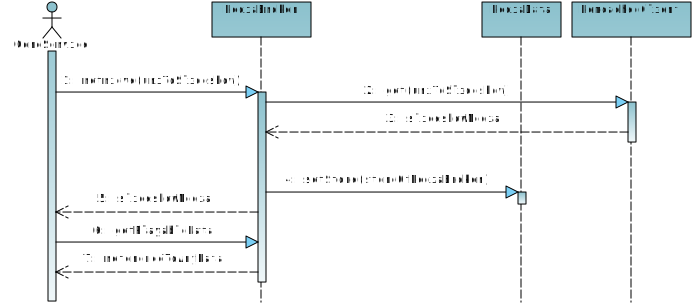
\includegraphics[width=.9\textwidth]{images/Handling_of_Media_Objects_read.pdf}
    \caption{Sequenzdiagramm über das Lesen von Medienobjekten}
    \label{fig:images_Handling_of_Media_Objects_read}
  \end{figure}
  
% subsection explizite_umsetzung_des_datenfluss (end)

\subsection{Extraktion der Komponenten als Dienste} % (fold)
\label{sub:extraktion_der_komponenten_als_dienste}

  Möglichkeit Komponenten auf unterschiedlichen Plattformen und physikalischen Umgebungen lauf zu lassen. Dazu Realisierung als Web Services. Eignet sich dadurch auch gut für die Verwendung von BPEL. Umsetzung muss aber nicht als Web Service erfolgen. Definition der Schnittstellenbeschreibung unabhängig von Web Service Technologie. Alternativ wäre auch eine Umsetzung über REST möglich~\citep{fielding00rest}, wobei REST-Architekturen nicht vollständig die  Eigenschaften von Diensten nach~\citep{service_oriented_computing} umsetzen können. Wichtig hier: Komponenten und Schnittstellen Definition sind agnostisch gegenüber der konkreten Technologie sie in verteilten Umgebungen bereitzustellen. 
  
  Integration einer Datenbank um Dienste wieder finden zu können, daher \verb!ServiceRegistry!.

% subsection extraktion_der_komponenten_als_dienste (end)
  
\subsection{Probleme und Lösungen} % (fold)
\label{sub:probleme_und_loesungen_architektur}

  - Welche Probleme sind aufgetaucht?
  - Wie wurden diese gelöst?
  - Auswirkungen auf die Architektur!
  - Workflow ohne externes Messaging System möglich!?
  
  Keine adäquate Fehlerbehandlung.
  
  Verteilte Ausführung der Komposition setzt ebenfalls eine verteilte Hinterlegung des aktuell Fortschritts der Ausführung voraus.
  
  Keine Möglichkeit zur asynchronen Ausführung von einzelnen Diensten bis jetzt implementiert. Ist nicht immer angemessen abhängig vom Art des Dienstes, doch mit unter notwendig (\textbf{Stichwort}: \emph{Streaming-Dienste}).
  
  Die bisherige Umsetzung der Komposition der einzelnen Dienste ist nur wenig flexibel und eignet sich wahrscheinlich nicht für Realisierung von komplexeren Szenarien. Dafür wäre im jeden Fall die Umsetzung auf Basis eines Zustandsautomaten notwenig, viel eher sollte aber die Verwendung einer etablierten Prozessbeschreibungssprache in Betracht gezogen werden. Dazu sind jedoch weitere Betrachtungen notwendig, wie sie unter anderem in~\citep{samma08} gemacht wurden.

  Bereits bei dieser einfachen Anwendung besteht auch ein Bedarf nach Synchronisation. Die Tranformer-Komponente, die die Diashow und das Musikstück verarbeitet muss dabei beide Medien synchronisieren. Es findet hier allerdings nur eine implizite Synchronisation statt, da sie in keiner Weise spezifiziert wurde. Des Weiteren wird sie auf Tranformer-Seite durchgeführt, was der Synchronisation durch Multiplex-Datenströme nach Steinmetz entspricht~\citep[S. 609]{multimedia_technologie} (siehe auch Abschnitt \ref{par:besonderheiten_bei_verteilten_umgebungen}).

% subsection probleme_und_loesungen_architektur (end)

% section realisierung_der_architektur (end)

\section{Realisierung des Szenario} % (fold)
\label{sec:realisierung_des_szenario}

  - Nerstrand Projekt
  - wichtige Punkte beschreiben
  - top-down Ansatz

\subsection{Extrahierte Anforderungen} % (fold)
\label{sub:extrahierte_anforderungen}

% subsection extrahierte_anforderungen (end)

\subsection{Vorgehen} % (fold)
\label{sub:vorgehen_szenario}

  - wie wurde bei der Umsetzung des Anwendungsszenario vorgegangen?

% subsection vorgehen_szenario (end)

\subsection{Probleme und Lösungen} % (fold)
\label{sub:probleme_und_loesungen_szenario}

  - Welche Probleme sind aufgetaucht?
  - Wie wurden diese gelöst?
  - Auswirkungen auf die Architektur!

% subsection probleme_und_loesungen_szenario (end)

% section realisierung_des_szenario (end)

% chapter prototypische_realisierung (end)
\chapter{Validierung der Architektur} % (fold)
\label{cha:validierung_der_architektur}

- Vorgehen bei der Validierun darstellen
- Quellen, die dieses Vorgehen beschreiben
- Vorgehen muss noch gefunden werden (!!)
- BPEL/Orchestrierung/Choreographie mit Quellenangaben erläutern. Auswirkungen auf die ursprüngliche Konzeption der Architektur darlegen (Messaging System vs Aufruf vom Workflow System)

% chapter validierung_der_architektur (end)
\chapter{Fazit} % (fold)
\label{cha:fazit}

  In dieser Arbeit wurde die Konzeption, prototypische Implementierung sowie die Validierung einer dienstorientierten Architektur für Multimediaanwendungen behandelt. Bei der Konzeption wurde zunächst ersichtlich, dass eine dienstorientierte Architektur eine Vielzahl von unterschiedlichen Komponenten aufweist, von denen jede einzelne bereits ein gewisses Maß an Komplexität aufweist. Unter der Hinterzunahme der zusätzlichen Eigenschaften, die die Integration von Multimedia gefordert hat, entstand eine komplexe Gesamtarchitektur.
  
  Durch diese Komplexität war es notwendig die jeweiligen Komponenten zunächst isoliert zu betrachten und im Anschluss in den größeren Kontext einzuordnen. Durch dieses Vorgehen wurde zum einen ein sehr viel besseres Verständnis über COSIMA entwickelt, zum anderen lassen sich die Komponenten in weiteren Arbeiten dadurch einzeln leichter betrachten.
  
  In seiner Gesamtheit weist das COSIMA-Projekt schon ein sehr hohes Maß an Vollständig\-keit auf. Die wesentlichen Aspekte sind durchweg bekannt und entsprechend diskutiert worden. Lediglich in vertikaler Richtung fehlt es Aspekten, wie der Synchronisation von Medien oder der Behandlung von Metadaten noch an Substanz.
  
  Entsprechend der Konzeption konnte auch die Implementierung in horizontaler Ebene fast vollständig umgesetzt werden. Auch hier wurde für nachfolgende Arbeiten diese Grundlage geschaffen. Dies wurde vor allem auch durch das iterative Entwicklungsvorgehen und durch den Einsatz eines szenariobasierten Ansatzes begünstigt. Durch den vermehrten Einsatz von etablierten Entwurfsmustern und Entwicklungsparadigmen sowie der Verwendung der Programmiersprache Java während der Implementierung wurde auch in diesem Teil eine solide Basis für Folgeprojekte geschaffen.
  
  Es lässt sich also festhalten, dass die beiden aufgestellten Ziele im Rahmen der gestellten Aufgaben für diese Arbeit als erfüllt gelten können. Dennoch müssen einige Punkte kritisch angemerkt werden.
  
  Die Nichtverwendung einer etablierten Prozessbeschreibungssprache stellt eines der Hauptprobleme dar. Zwar erlaubt die gewählte Lösung in dieser Arbeit ein besseres Verständnis über die internen Abläufe bei der Servicekomposition, für eine langfristige Weiterentwicklung sollte diese Komponente jedoch ausgetauscht werden. Stattdessen sollte die Eignung und Anpassung bestehender Lösungen weiterverfolgt werden, wie sie bereits bei \citep{samma08} begonnen wurde.
  
  Ebenfalls nur rudimentär ist die Integration von Synchronisation durchgeführt worden. Es wurde vor allem klar, dass es sich dabei um ein sehr komplexes Themengebiet handelt. In \citep{antons09} findet aber bereits eine intensivere Auseinandersetzung mit der Einbindung von Synchronisation in das COSIMA-Projekt statt. In Zukunft sollten Arbeiten die dort gefundenen Ergebnisse mit der hier vorgestellten Implementierung in Einklang bringen.
  
  Der letzte Punkt, der weitestgehend ausgelassen wurde, ist die Betrachtung von Metadaten. Da dieser aber nicht zur essentiellen Funktionalität des umgesetzten Szenarios gehört, wurde bisher nur eine Schnittstelle vorgesehen. In \citep{lehmann09} findet sich eine dedizierte Betrachtung dieses Themas im Kontext von COSIMA.
  
  Zu den anderen Punkten kann festgehalten werden, dass sie trotz ihres prototypischen Charakters durchaus so implementiert sind, dass sie sich auch für den Einsatz in Folgeprojekten eignen.
  
  Abschließend lässt sich festhalten, dass das gesamte COSIMA-Projekt einen innovativen und breiten Themenbereich im Rahmen der Medieninformatik bietet. Nachdem in dieser Arbeit zum ersten Mal eine funktionierende Implementierung der grundlegenden Architektur geliefert wurde, haben künftige Arbeiten in diesem Bereich eine robuste Basis zur Hand, um in den unterschiedlichen Teilbereichen des Projekts in die Tiefe gehen zu können.

% chapter fazit (end)

\appendix

% \nocite{*}
\bibliography{std/bibliography}

% Einbinden des Anhangs
%!TEX root = /Users/dbreuer/Documents/Work/_FH/_Master/master_thesis/Main/Master Thesis.tex

\chapter{Weitere Listings} % (fold)
\label{cha:more_listing}

  In diesem Anhang finden sich solche Listings, die eine zu umfangreich waren, um im laufenden Text untergebracht zu werden, dennoch aber von Interesse während des Lesens der Arbeit sind und daher nicht nur auf der Begleit-CD zu finden sein sollten.

  \lstinputlisting[caption=\texttt{WorkflowElement}-Klasse,label=lst:workflow_element,language=Java,firstline=12]{../code/COSIMA/src/main/java/de/fhkoeln/cosima/workflow/WorkflowElement.java}

  \lstinputlisting[caption=\texttt{RemoteWorkflowEngine}-Klasse,label=lst:remote_workflow_engine,language=Java,firstline=12]{../code/COSIMA/src/main/java/de/fhkoeln/cosima/workflow/RemoteWorkflowEngine.java}
  
  \lstinputlisting[caption=Die vollständige \texttt{AbstractComponent}-Klasse,label=lst:abstract_component_final,language=Java,firstline=12]{../code/COSIMA/src/main/java/de/fhkoeln/cosima/components/AbstractComponent.java}
    
% chapter more_listing (end)

%!TEX root = /Users/dbreuer/Documents/Work/_FH/_Master/master_thesis/Main/Master Thesis.tex

\chapter{Architekturdarstellungen} % (fold)
\label{cha:architekturdarstellungen}

  - Auszüge aus UML-Diagrammen

% chapter architekturdarstellungen (end)

% Einbinden der Eigenständigkeitserklärung
%!TEX root = /Users/dbreuer/Documents/Work/_FH/_Master/master_thesis/Main/Master Thesis.tex

\chapter*{Erklärung}\label{chap:erklaerung}

Ich versichere, die von mir vorgelegte Arbeit selbständig verfasst zu haben.\\ \\
Alle Stellen, die wörtlich oder sinngemäß aus veröffentlichten oder nicht veröffentlichten Arbeiten anderer entnommen sind, habe ich als entnommen kenntlich gemacht. Sämtliche Quellen und Hilfsmittel, die ich für die Arbeit benutzt habe, sind angegeben.\\ \\
Die Arbeit hat mit gleichem Inhalt bzw. in wesentlichen Teilen noch keiner anderen Prüfungsgbehörde vorgelegen.

\vspace{4cm}

\begin{flushright}
  -----------------------------------------------------------------\\
  Dirk Breuer --- Köln, den \today
\end{flushright}


% Unbeschriftetes Abschlussblatt
\include{std/empty}

\end{document}
